\documentclass[a4paper,11pt]{article}
\usepackage[T1]{fontenc}
\usepackage[utf8]{inputenc}
\usepackage{lmodern}
\usepackage[margin=2.4cm]{geometry}
\usepackage{amsmath,amssymb}
\usepackage{graphicx}
\usepackage{booktabs}
\usepackage{tabularx}
\usepackage{longtable}
\usepackage{xcolor}
\usepackage{listings}
\usepackage{tikz}
\usetikzlibrary{arrows.meta,positioning,fit,calc}
\usepackage{siunitx}
\usepackage{caption}
\usepackage[hidelinks]{hyperref}

\graphicspath{{figures/}}
\sisetup{group-separator={,},group-minimum-digits=4}

\definecolor{codebg}{HTML}{F6F5F2}
\definecolor{codekw}{HTML}{2A78D6}
\definecolor{codecm}{HTML}{6E6D68}
\definecolor{codestr}{HTML}{B4501F}
\lstset{
  language=Python, basicstyle=\ttfamily\footnotesize, backgroundcolor=\color{codebg},
  keywordstyle=\color{codekw}\bfseries, commentstyle=\color{codecm}\itshape,
  stringstyle=\color{codestr}, frame=none, columns=fullflexible, keepspaces=true,
  breaklines=true, showstringspaces=false, xleftmargin=0.6em, framexleftmargin=0.6em,
  aboveskip=0.8em, belowskip=0.8em, upquote=true
}
\usepackage{xurl}
\DeclareUrlCommand\code{\urlstyle{tt}}
\newcommand{\etagt}{\eta_{GT}}
\newcommand{\etao}{\eta_{o}}
\newcommand{\EI}[1]{\mathrm{EI}_{\mathrm{#1}}}

\title{PhlyGreen Technical Manual: Engine Decks and Emissions\\[4pt]
\large Gas turbine, turbofan, propeller and emission-index models: physics, surrogates and usage}
\author{PhlyGreen development team\\Sapienza University of Rome}
\date{Code state: November 2026, branch \texttt{main}}

\begin{document}
\maketitle

\begin{abstract}
\noindent This manual documents the engine decks of PhlyGreen and the emission-index models
built on the same infrastructure. An engine deck is a table of engine performance generated
offline by a physical model and replaced at run time by a fitted surrogate. We describe four
models. The turboshaft deck gives the thermal efficiency of a gas turbine as a function of
altitude, Mach number and power fraction. The turbofan deck gives the overall efficiency, the
thrust-specific fuel consumption and the thrust lapse of a high-bypass engine. The propeller
models give the propulsive efficiency, either from the Hamilton-Standard charts or from a
fitted map. The emission-index surrogates give the NO$_x$, CO and unburned-hydrocarbon indices
of a turboprop and of a turbofan combustor, computed by a chemical reactor network. For each
model we give the physical model, the surrogate, its accuracy, the way the sizing uses it and
its limits. Every number in the manual comes from running the code. The scripts that produce
the numbers and the figures are in \code{manuals/engine-decks/scripts/}.
\end{abstract}

\tableofcontents
\newpage

%% ======================================================================================
\section{Scope and overview}\label{sec:scope}
%% ======================================================================================

PhlyGreen sizes an aircraft with an iterative take-off-weight loop. Each pass flies the mission
and needs, at every integration point, the fuel power that produces the required propulsive
power. That ratio is the product of the component efficiencies of the powertrain. In the
simplest models (Class~I) each efficiency is a constant. In the models of this manual
(Class~II) the gas-turbine and propeller efficiencies depend on the operating point.

Running a thermodynamic cycle at every integration point would be too slow. Therefore
PhlyGreen never runs a cycle during a design. The cycle is run offline over a grid of operating
points, the results are stored in a CSV file, and a surrogate (a radial-basis-function
interpolant, RBF) is fitted to that file and stored as a pickle artifact. At run time only the
artifact is loaded. We call the offline table an \emph{engine deck}, and the fitted artifact its
\emph{surrogate}.

The manual covers four models:
\begin{itemize}
\item \textbf{Gas turbine (turboshaft).} A two-shaft pyCycle cycle gives the thermal efficiency
  $\etagt$ versus altitude, Mach number and power fraction. A size-scaling law corrects the
  efficiency for engines smaller or larger than the reference.
  Section~\ref{sec:gt}.
\item \textbf{Turbofan.} A high-bypass pyCycle cycle gives the overall efficiency $\etao$, the
  TSFC and the thrust lapse versus altitude, Mach number and thrust fraction. The turbofan is
  sized on thrust rather than shaft power. Section~\ref{sec:tf}.
\item \textbf{Propeller.} The Hamilton-Standard chart model, and an RBF map fitted to a
  blade-element dataset. Section~\ref{sec:prop}.
\item \textbf{Emission indices.} A Cantera chemical reactor network (CRN) turns the combustor
  inlet state of a cycle into NO$_x$, CO and unburned-hydrocarbon (UHC) indices. Two
  surrogates ship: one for a PW127-class turboprop and one for a CFM56-class turbofan. The
  climate module integrates them over the mission. Sections~\ref{sec:em-physics},
  \ref{sec:em-surrogate} and~\ref{sec:em-climate}.
\end{itemize}

The powertrain architecture (how the component efficiencies combine into power ratios) belongs
to the companion manual \emph{PhlyGreen Technical Manual: Powertrain Architectures}. We
summarize it in Section~\ref{sec:interface}. Fuel-cell and battery efficiencies belong to the
fuel-cell and battery manuals.

\paragraph{Where the code lives.} Table~\ref{tab:files} lists the files. The decks are read by
\code{Powertrain._build_efficiencies}, which runs at the end of \code{Powertrain.SetInput}. The
emission surrogates are read by \code{ClimateImpact}.

\begin{table}[htbp]
\centering\small
\caption{Source files of the engine decks and emission models (paths relative to
\texttt{trunk/PhlyGreen/Systems/Powertrain/} unless stated otherwise).}\label{tab:files}
\begin{tabularx}{\textwidth}{@{}lX@{}}
\toprule
File & Content \\
\midrule
\code{efficiency.py} & \code{OperatingPoint}, \code{EfficiencyModel} and its implementations, among them \code{GasTurbineEfficiencyModel}, \code{TurbofanEfficiencyModel}, \code{HamiltonPropellerEfficiency}, \code{PropellerSurrogateEfficiency} \\
\code{Powertrain.py} & \code{_build_efficiencies}, \code{eta}, \code{PowerLapse}, \code{ThrustLapse}, \code{SizingDenominator}, \code{WeightPowertrain}, \code{report_class_ii_sizing}, \code{report_turbofan_sizing} \\
\code{gas_turbine_surrogate.py} & \code{GasTurbineResponseSurface}, size scaling, ISA pressure lapse \\
\code{train_gas_turbine_surrogate.py} & offline fit of \code{data/GT_Engine_Model_Complete.pkl} \\
\code{turbofan_surrogate.py} & \code{TurbofanResponseSurface} \\
\code{train_turbofan_surrogate.py} & offline fit of \code{data/Turbofan_Engine_Model.pkl} \\
\code{propeller_hamilton.py}, \code{propeller_hamilton_tables.py} & Hamilton-Standard model and its chart data \\
\code{propeller_surrogate.py} & \code{PropellerSurrogate} (RBF fitted from \code{data/propeller_data_rbf.csv}) \\
\code{emissions_surrogate.py} & \code{EmissionSurrogate}, \code{default_model_path} \\
\code{train_emission_surrogate.py} & offline fit of the emission artifacts \\
\code{emissions_pipeline/} & offline emission pipeline: CRN (\code{crn/}), PW127 deck and calibration, the two build scripts, notes \\
\code{data/} & decks (\code{Single_spool_GT.py}, \code{HBTF_turbofan.py}), maps (CSV), artifacts (pickle), \code{README.md} \\
\code{trunk/PhlyGreen/ClimateImpact/ClimateImpact.py} & Filippone NO$_x$ correlation and the surrogate integration over the mission \\
\code{trunk/PhlyGreen/config/sections.py} & \code{EnergyConfig} (deck selection and ratings), \code{ClimateImpactConfig} \\
\bottomrule
\end{tabularx}
\end{table}

\paragraph{Reference configurations.} All numbers in this manual come from the scripts in
\code{manuals/engine-decks/scripts/}. The aircraft designs use the configurations of
\code{trunk/examples/common.py}:
\begin{itemize}
\item \textbf{TP}: \code{traditional_config()}, an ATR-like turboprop with \SI{4560}{kg}
  payload, a \SI{750}{nmi} mission and a \SI{220}{nmi} diversion, a constant gas-turbine
  efficiency of 0.22, a constant propulsive efficiency of 0.9 and a gearbox efficiency of 0.96.
  The Class-II variants replace the gas turbine or the propeller model and keep everything else.
\item \textbf{TF}: \code{turbofan_config()}, an A320-class turbofan with \SI{14250}{kg}
  payload, a \SI{3000}{nmi} mission, a \SI{200}{nmi} alternate and a \SI{30}{min} hold, the
  compressible drag polar and a nominal sea-level-static thrust of \SI{240.2}{kN}.
\end{itemize}
The mission emissions add a \code{ClimateImpactConfig(H=100, N=1.6e7, Y=30)} with the NO$_x$
model under study, as in \code{examples/24_gt_emissions_surrogate.py}.

\paragraph{Offline toolchain.} The decks need pyCycle (installed as \code{om-pycycle}) and
OpenMDAO; the emission pipeline also needs Cantera. The run-time models need only numpy, scipy,
scikit-learn and pandas. In the environment used for this manual pyCycle~4.4.0,
OpenMDAO~3.44.0 and Cantera~3.2.0 are installed, the versions that
\code{data/README.md} lists for the shipped artifacts. Therefore we could re-run the
turboshaft deck and the CRN to check the shipped data (Sections~\ref{sec:gt-conv}
and~\ref{sec:em-physics}). We did not regenerate or overwrite any artifact.

%% ======================================================================================
\section{How a deck enters the sizing}\label{sec:interface}
%% ======================================================================================

\subsection{The powertrain graph}
The powertrain is a graph of converters, combiners and splits. For a given propulsive power
$P_p$ the graph returns the normalized power ratios: \code{PRatio[0]} $= P_f/P_p$ is the fuel
power, \code{PRatio[1]} the gas-turbine shaft power and \code{PRatio[5]} the battery power.
For the conventional chain fuel $\to$ gas turbine $\to$ gearbox $\to$ propeller,
\begin{equation}
  \frac{P_f}{P_p} = \frac{1}{\etagt\,\eta_{GB}\,\eta_{P}} .
  \label{eq:chain}
\end{equation}
The mission integrates the fuel flow $\dot m_f = P_p\,(P_f/P_p)/E_f$, with $E_f$ the fuel
specific energy of \code{EnergyConfig.Ef}. The graph itself, the hybrid architectures and the
legacy matrix solvers are described in \emph{PhlyGreen Technical Manual: Powertrain
Architectures}. For this manual it is enough that every efficiency in~\eqref{eq:chain} is read
through one call, \code{Powertrain.eta(component, alt, vel, pwr)}, at the altitude, true
airspeed and power of the current point. The power \code{pwr} is the power through the
component itself: the shaft output for the gas turbine, the shaft input for the propeller and
the input for the gearbox. For the chain of~\eqref{eq:chain} these are
$P_p/(\eta_{GB}\,\eta_P)$, $P_p/\eta_P$ and $P_p/(\eta_{GB}\,\eta_P)$.

The component powers depend on the efficiencies, so \code{Powertrain._solve_at_component_powers}
finds them by a damped fixed-point iteration. The first pass evaluates every model at $P_p$ and
solves the graph. Each further pass moves the powers the models are read at towards the
component powers of the last solution, by a fraction \code{relax} of the difference. The
fraction starts at 1 and is halved whenever the step of any power-dependent component changes
sign. The iteration stops when the solved powers match those the models were read at within
$10^{-6}\,|P_p|$, and warns if 50 passes are not enough. The damping matters for a propeller at
low power, whose efficiency rises steeply with its shaft power: there the plain update
$P \leftarrow P_p/\eta(P)$ overshoots and oscillates. When every model of the graph is a
constant, the first solution is returned, so a Class-I design is unaffected by the iteration.

\subsection{The efficiency interface}
\code{efficiency.py} defines an \code{OperatingPoint} (altitude [m], velocity [m/s TAS],
power [W], optional rpm and voltage) and an abstract \code{EfficiencyModel} with one method,
\code{eta(op)}. \code{Powertrain._build_efficiencies} builds one model per component from the
\code{EnergyInput} keys, as Table~\ref{tab:selection} lists. A model that is not selected is a
\code{ConstantEfficiency}. When the constant itself is missing, the defaults are 0.30 for the
gas turbine and 0.85 for the propeller, each with a \code{UserWarning}, and 1.0 for the
gearbox.

\begin{table}[htbp]
\centering\small
\caption{How \texttt{Powertrain.\_build\_efficiencies} selects a model. Keys of
\texttt{EnergyConfig}; legacy dictionary keys in Table~\ref{tab:inputs}.}\label{tab:selection}
\begin{tabularx}{\textwidth}{@{}p{3.6cm}p{3.0cm}X@{}}
\toprule
Component & Selector value & Model \\
\midrule
gas turbine & \code{'constant'} (default) & \code{ConstantEfficiency(eta_gas_turbine)} \\
 & \code{'ResponseSurface'} & \code{GasTurbineEfficiencyModel}; nominal \code{gt_design_power} [W], or the sized rating when it is not set \\
 & \code{'Turbofan'} & \code{TurbofanEfficiencyModel}; needs \code{turbofan_design_thrust} [N]; gearbox and propeller forced to 1.0 \\
propeller & \code{'constant'} (default) & \code{ConstantEfficiency(eta_propulsive)} \\
 & \code{'Hamilton'} & \code{HamiltonPropellerEfficiency}; needs \code{aircraft.PropellerInput} geometry \\
 & \code{'Surrogate'} or \code{'RBF'} & \code{PropellerSurrogateEfficiency} at \code{propeller_rpm} (default 1200) \\
\bottomrule
\end{tabularx}
\end{table}

A Class-II gas turbine or turbofan reads its map at a fraction of a \emph{nominal rating}. An
engine cannot resize itself at every integration point, so the nominal rating is fixed for each
flight of the mission. For the turbofan it is an input, \code{turbofan_design_thrust}. For the
gas turbine it is either an input, \code{gt_design_power}, or, when that input is not set, the
rating of the engine sized by the weight loop (Section~\ref{sec:gt-sizing}). After the design,
\code{report_class_ii_sizing} and \code{report_turbofan_sizing} compare the nominal with what
the mission required (Sections~\ref{sec:gt-sizing} and~\ref{sec:tf-sizing}).

\paragraph{Engine count.} The model has one engine count, \code{powertrain.n_engines}.
\code{Powertrain.SetInput} reads it from the key \texttt{Number of Engines} of
\code{aircraft.PropellerInput}, with a default of 2 when the key or the dictionary is absent. The
legacy Hamilton key \texttt{N\_ENGINES} is accepted, with a deprecation warning, when
\texttt{Number of Engines} is missing. The Class-II gas-turbine, motor and propeller models,
the Hamilton propeller and the Filippone correlation of the climate module all divide the
power or the fuel flow by this count. The typed configuration has no propeller section, so a
count other than 2 is set through the dictionary on the aircraft before \code{configure}
(Section~\ref{sec:usage}). The engine count matters for the gas turbine because the size scaling
of Section~\ref{sec:gt-scaling} uses the power per engine.

%% ======================================================================================
\section{Gas turbine (turboshaft)}\label{sec:gt}
%% ======================================================================================

\subsection{Physical model: the pyCycle deck}\label{sec:gt-deck}
\code{data/Single_spool_GT.py} defines a two-shaft turboshaft in pyCycle with CEA
thermodynamics: inlet, compressor (map \code{AXI5}), burner (fuel \code{JP-7}), high-pressure
turbine (map \code{LPT2269}) on the gas-generator shaft, free power turbine (map \code{LPT2269})
on the output shaft, and a convergent nozzle. The design point is sea-level static with a shaft
power of \SI{2750}{hp}, a turbine inlet temperature of \SI{2370}{\degree R}, a compressor pressure
ratio of 13.5, component efficiencies of 0.86 (compressor), 0.885 (gas-generator turbine) and
0.915 (power turbine), a burner pressure loss of 3\,\% and a nozzle pressure ratio of 1.2. At this
design point our re-run (Section~\ref{sec:gt-conv}) gives an inlet flow of
\SI{16.83}{lbm/s}, a fuel flow of \SI{0.1365}{kg/s} and a thermal efficiency of 0.3495.

Off design, three balances close the cycle: the fuel-to-air ratio is varied to reach the
requested shaft power, the gas-generator speed to balance its shaft, and the inlet flow to
match the nozzle throat area of the design. The thermal efficiency of a point is
\begin{equation}
  \etagt = \frac{P_{shaft}}{\dot m_f\,\mathrm{LHV}}, \qquad \mathrm{LHV} = \SI{43}{MJ/kg}.
  \label{eq:etagt}
\end{equation}
The sweep covers four altitudes (0, \num{10000}, \num{20000} and \SI{30000}{ft}), four Mach
numbers (0.01, 0.2, 0.4, 0.6) and five power fractions between 0.3 and 1.0 of the power available
at the altitude, $P_{avail} = P_{des}\,\delta(h)$, with $\delta$ the ISA pressure ratio. The power
fraction, not the power, is stored. This makes the map independent of engine size. The script
writes 80 rows to \code{GT_Universal_Map.csv}, with the target and the delivered shaft power of
every point.

\subsection{Convergence of the map}\label{sec:gt-conv}
The Newton solver of the deck is set not to raise when a sub-solve fails
(\code{reraise_child_analysiserror = False}), so a stalled solve returns a state as if it had
converged. The generator therefore checks every point itself. A point is accepted only if three
off-design balances are closed within 0.1\,\%: the delivered shaft power against the target, the
net power of the gas-generator shaft against the target power, and the nozzle throat area
against the design area. Each (altitude, Mach) column is solved from full power downwards, and
each point is warm-started from its converged neighbour. When no warm start converges, the
generator walks the power target from the neighbour in 4 and then 10 steps. A point that still
fails stops the script, and the trainer \code{train_gas_turbine_surrogate.py} refuses a map with
a row whose delivered power is more than 0.1\,\% away from its target.

The static column is solved at Mach 0.01. The comment in \code{Single_spool_GT.py} states that
pyCycle's \code{FlightConditions} is singular at Mach 0 exactly, so that Newton does not move and
the fuel-to-air ratio stays at its initial guess. Our check confirms it: at sea level, Mach 0
and \SI{2750}{hp}, a solve from fresh guesses ends with FAR $= 0.017$, the initial guess, and
delivers \SI{1681}{hp}.

\code{scripts/check_gt_deck.py} re-runs the generator's own sweep and records the closure
errors of every accepted point. The re-run reproduces every efficiency of the shipped CSV to
$6\times10^{-17}$. Over the 80 points the largest errors are $1.8\times10^{-4}$ on the delivered
power, $7.3\times10^{-5}$ on the gas-generator shaft and $7.6\times10^{-4}$ on the nozzle area,
all below the tolerance of $10^{-3}$. The fuel-to-air ratio ranges from 0.0076 to 0.0179. The
shipped CSV itself records a largest power error of $1.8\times10^{-4}$. The emission pipeline
runs the same deck with the same acceptance test on the delivered power
(Section~\ref{sec:em-pw127}).

\begin{figure}[htbp]
\centering
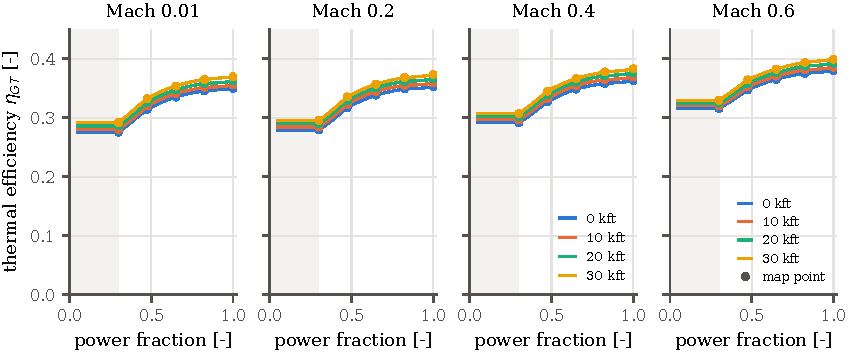
\includegraphics[width=\textwidth]{gt_map.pdf}
\caption{Turboshaft surrogate at the reference size (\SI{2750}{hp}): thermal efficiency versus
power fraction at four Mach numbers and four altitudes. Dots: map points, all converged. The
grey band is below the training range, where the surrogate returns the value at a fraction of
0.3.}
\label{fig:gt-map}
\end{figure}

\subsection{The surrogate}\label{sec:gt-surrogate}
\code{train_gas_turbine_surrogate.py} standardizes the inputs (altitude [ft], Mach, power
fraction) with a scikit-learn \code{StandardScaler} and fits a scipy \code{Rbf} with the
\code{linear} kernel and no smoothing. The pickle stores the scaler and the RBF, a dry-mass
RBF (Section~\ref{sec:gt-lapse}), the reference power (\SI{2750}{hp}) and the size-scaling
exponent.

With no smoothing the RBF is an interpolant: at the 80 training points its error is
$1.7\times10^{-16}$ at most. This says nothing about the error between points. To measure it we
refitted the RBF 80 times with the same settings, each time leaving one point out, and
predicted that point (\code{compute_data.py}, in memory; the artifact is not touched). The
leave-one-out error of $\etagt$ has a mean absolute value of 0.0046, an rms of 0.0070 and a
maximum of 0.025. The map spans $\etagt$ from 0.276 to 0.399.

At run time \code{GasTurbineResponseSurface.predict(design_hp, alt_ft, mach, required_hp)}
works per engine:
\begin{enumerate}
\item it computes the available power $P_{avail} = P_{des}\,\delta(h)$ and flags the point as
  power-limited when the requirement exceeds it (the power is then capped at $P_{avail}$);
\item it forms the power fraction $P/P_{avail}$;
\item it clips altitude, Mach number and fraction to the training box stored in the pickle
  (\code{input_ranges}: 0 to \SI{30000}{ft}, Mach 0.01 to 0.6, fraction 0.3 to 1.0), with a
  \code{RuntimeWarning} the first time each coordinate is clipped;
\item it evaluates the RBF and applies the size scaling of Section~\ref{sec:gt-scaling}, then
  clips the result to $[0.01, 0.45]$.
\end{enumerate}
Below a fraction of 0.3 the surrogate therefore returns the value at 0.3: at \SI{20000}{ft} and
Mach 0.4 it gives 0.302 at fractions of 0.05, 0.1, 0.2 and 0.3 alike. A real turboshaft loses
more efficiency towards idle, so the value is optimistic there. When the inputs are invalid or
the evaluation fails, \code{predict} returns $\etagt = 0.30$ with a \code{RuntimeWarning}.

\code{GasTurbineEfficiencyModel.eta(op)} converts the operating point to the inputs of
\code{predict}: the Mach number from the ISA speed of sound, the altitude in feet, and the
nominal and required powers in horsepower divided by \code{n_engines}. The required power is
the shaft output of the gas turbine (Section~\ref{sec:interface}), the same quantity that
\code{report_class_ii_sizing} checks against the available power.

\subsection{Size scaling}\label{sec:gt-scaling}
The map describes one engine. A smaller turboshaft has larger relative losses. PhlyGreen scales
the losses with the nominal power per engine,
\begin{equation}
  1 - \etagt = (1 - \eta_{ref})\left(\frac{P_{ref}}{P_{des}}\right)^{n},
  \label{eq:scaling}
\end{equation}
with $\eta_{ref}$ the map value and $P_{ref} = \SI{2750}{hp}$. \code{calibrate_scaling_exponent}
fits $n$ by least squares to nine (power, SFC) pairs embedded in the code, converted to
efficiency with $\eta = 2544.43/(\mathrm{SFC}\cdot 18400)$, and referenced to the
\SI{2500}{shp} row. The comments of \code{Single_spool_GT.py} name the engines (Allison 250,
Arriel, PT6A, CT7, T700, T64 and a Soloviev D-25V) and give jet-engine.net as the origin. The
fit gives $n = 0.0556$; the pickle stores the same value.

Figure~\ref{fig:gt-scaling}(a) shows the data and the fit. Eight points follow the law within
0.015. The \SI{5500}{shp} row (SFC 0.64, $\eta = 0.216$) lies far below it and pulls $n$ down: without it the fit gives $n = 0.068$.
Figure~\ref{fig:gt-scaling}(b) shows the effect at \SI{20000}{ft}, Mach 0.4 and 70\,\% power:
$\etagt$ rises from 0.281 at \SI{300}{hp} to 0.364 at the reference size and 0.401 at
\SI{8000}{hp}. A larger nominal power therefore raises the efficiency of every point, which
matters for the sizing workflow of Section~\ref{sec:gt-sizing}.

\begin{figure}[htbp]
\centering
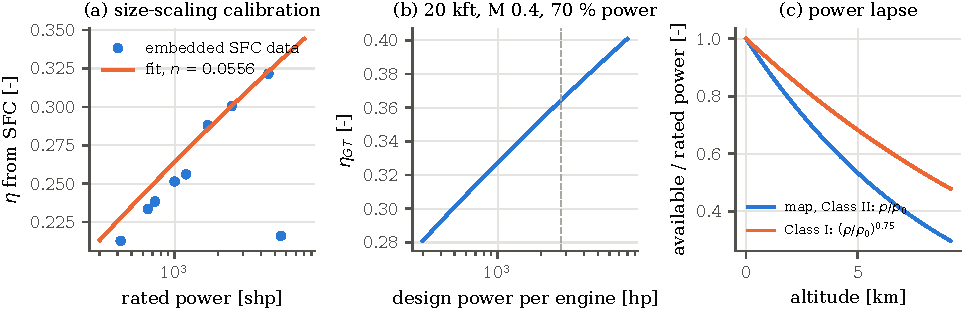
\includegraphics[width=\textwidth]{gt_scaling.pdf}
\caption{(a) Efficiency from the embedded SFC data and the fitted loss scaling. (b) Surrogate
efficiency versus nominal power per engine. (c) Available power over rated power: the ISA
pressure ratio, which is the map coordinate and \texttt{Powertrain.PowerLapse} with the Class-II
map, and the density lapse that \texttt{PowerLapse} returns otherwise.}
\label{fig:gt-scaling}
\end{figure}

\subsection{Power lapse and dry mass}\label{sec:gt-lapse}
The map defines its power fraction against $P_{des}\,\delta(h)$, with $\delta = p/p_0$ the ISA
pressure ratio, so $\delta$ is a coordinate of the map. The constraint diagram and
\code{WeightPowertrain} rate the engine with \code{Powertrain.PowerLapse}, which depends on the
gas-turbine model. With the Class-II map (\code{gas_turbine_has_map_lapse}) it returns the same
$\delta(h)$, with no Mach or DISA dependence, as in the deck. The engine is then rated with the
full power it has on the map. Otherwise it returns $(\rho/\rho_0)^{0.75}$, attributed in its
docstring to Ruijgrok, Eq.~(6.7-11)~\cite{ruijgrok}. At \SI{6096}{m} (\SI{20000}{ft}) the first
gives 0.460 and the second 0.624 (Figure~\ref{fig:gt-scaling}(c)). A constant-efficiency
engine is therefore rated with a lapse that falls more slowly than the coordinate of the
turboprop emission map, which matters for the emissions of Section~\ref{sec:em-path}.

With the Class-II map, \code{WeightPowertrain} rates the engine at the largest full-power
requirement on the map: the shaft power over $\delta(h)$ at every mission point
(\code{mission.Max_PEng_lapsed}) and the take-off or OEI shaft power referred to sea level by
$\delta$ at the take-off altitude (\code{Powertrain._map_lapse_engine_rating}). The available
power $\texttt{engineRating}\cdot\delta(h)$ then covers every mission point.

The pickle also holds an RBF of the dry engine mass versus design power, fitted to a WATE++-style
correlation of the design power (airflow $W = P/145$, OPR 15, component terms). The RBF
reproduces the correlation within 0.12\,\% between 300 and \SI{8000}{hp}; at \SI{2750}{hp} it
gives \SI{1357}{lb}. \code{GasTurbineEfficiencyModel} discards this mass. The powertrain mass
of the weight loop is always the rated power over the specific power \code{SPowerPT[0]}.

\subsection{Use in the sizing}\label{sec:gt-sizing}
The nominal power sets the map coordinate and the size scaling. There are two ways to fix it.

\paragraph{Nominal from the rating.} When \code{gt_design_power} is not set, the nominal follows
the rated power of the engine (\code{Weight._mission_and_powertrain}). At each take-off weight
of the Brent loop the nominal is seeded with $\texttt{DesignPW}\cdot W_{TO}$, the mission is
flown, \code{WeightPowertrain} rates the engine (Section~\ref{sec:gt-lapse}), the nominal is
set to that rating and the mission is flown again, until rating and nominal agree within
$10^{-7}$ (at most 20 passes). The engine that flies the mission is then the engine that is
weighed, and no mission point is power-limited. On TP with two engines this design closes at
$W_{TO} = \SI{17562}{kg}$ with \SI{1216.6}{kg} of fuel and a rating of \SI{5402}{kW}. The worst
ratio of shaft power to available power over the mission is 1.000, at the point that sets the
rating. The powertrain mass is \SI{1385}{kg}, against \SI{797}{kg} for the Class-I design, because
the steeper lapse $\delta$ refers the climb power to a larger sea-level rating. Without
\code{PropellerInput} the engine count defaults to 2, and the same design is obtained.

\paragraph{Explicit nominal.} \code{examples/16_class_ii_propulsion_sizing.py} fixes the
nominal by hand. We repeat its workflow on TP with two engines:
\begin{enumerate}
\item A Class-I pre-pass gives $W_{TO} = \SI{17843}{kg}$ and \code{DesignPW} $=
  \SI{163.3}{W/kg}$, hence a tentative nominal $P_{des} = \texttt{DesignPW}\cdot W_{TO} =
  \SI{2914}{kW}$.
\item The Class-II design with this nominal closes at $W_{TO} = \SI{17581}{kg}$, but
  \code{report_class_ii_sizing} reports it power-limited: the shaft power exceeds
  $P_{des}\,\delta(h)$ at 138 of the 238 mission points, by up to 85\,\%, and the minimum
  nominal is \SI{5404}{kW}. The report also warns that the nominal is 46\,\% below the sized
  rating, so that the flown engine is not the weighed one.
\item With $1.05$ times that minimum (\SI{5674}{kW}) the design closes at
  $W_{TO} = \SI{17568}{kg}$ with \SI{1218.8}{kg} of fuel, a rating of \SI{5406}{kW} and a worst
  load ratio of 0.953.
\end{enumerate}
The engine mass follows the rating, not the nominal. A nominal above the rating reads the map at
a lower load and a larger size without carrying the mass of that engine.
\code{report_class_ii_sizing} warns when the nominal differs from the rating by more than 5\,\%
(\code{GT_NOMINAL_RATING_RTOL}). The nominal of step~3 is 5.0\,\% above the rating, just inside
that tolerance, so no warning is issued.

Against the Class-I design (\SI{1939}{kg} of fuel at $\etagt = 0.22$), the Class-II engine with
the nominal from the rating burns 37\,\% less fuel. Its fuel-weighted mean efficiency over the
flown mission is 0.349, and $\etagt$ ranges from 0.295 to 0.390. Figure~\ref{fig:gt-mission}
shows the load and the efficiency along the mission.

\begin{figure}[htbp]
\centering
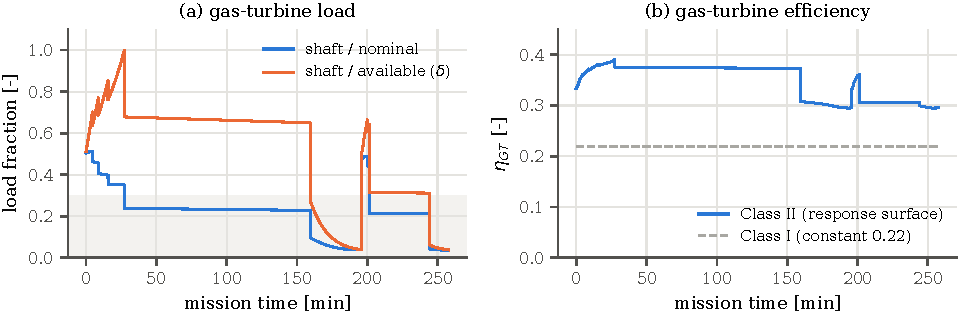
\includegraphics[width=\textwidth]{gt_mission.pdf}
\caption{TP with the Class-II gas turbine, nominal equal to the rating (\SI{5402}{kW}, two
engines). (a) Shaft power over the nominal and over the available power $P_{des}\,\delta(h)$,
which is the map coordinate. (b) Gas-turbine efficiency, compared with the constant 0.22 of the
Class-I design.}
\label{fig:gt-mission}
\end{figure}

%% ======================================================================================
\section{Turbofan}\label{sec:tf}
%% ======================================================================================

\subsection{Physical model: the pyCycle deck}\label{sec:tf-deck}
\code{data/HBTF_turbofan.py} vendors the high-bypass turbofan of the pyCycle example cycles
(Apache-2.0): a separate-flow two-spool engine with fan, low- and high-pressure compressors,
bleeds, burner, two turbines and two nozzles. The design point is \SI{35000}{ft}, Mach 0.8, net
thrust \SI{5900}{lbf}, maximum turbine inlet temperature \SI{2857}{\degree R}, bypass ratio
5.105, fan pressure ratio 1.685, compressor pressure ratios 1.935 and 9.369. The docstring
calls it CFM56-class. Every other point is an off-design solve on the frozen geometry, with the
bypass ratio as a balance variable against the bypass nozzle area.

At each flight condition the deck is solved twice: once at full throttle (temperature-limited)
for the available thrust $F_{max}(h, M)$, and once in \code{percent_thrust} mode for each thrust
fraction PC $\in\{0.30, 0.55, 0.80, 0.90, 1.00\}$ of it. The thrust fraction is therefore a native
coordinate and the map is independent of engine size. The overall efficiency and the TSFC are
\begin{equation}
  \etao = \frac{F\,V}{\dot m_f\,\mathrm{LHV}}, \qquad
  \mathrm{TSFC} = \frac{\dot m_f}{F} = \frac{V}{\etao\,\mathrm{LHV}}, \qquad
  \mathrm{LHV} = \SI{43}{MJ/kg},
  \label{eq:etao}
\end{equation}
and the thrust lapse is $\lambda_T = F_{max}(h, M)/F_{00}$, with $F_{00} = \SI{94.22}{kN}$ the
full-throttle thrust at sea level and Mach 0.001 (the deck does not converge at rest). $F_{00}$
is cached in \code{Turbofan_Universal_Map_F00.txt}.

The envelope is not a rectangle. Each Mach number carries the altitudes where it is flown
(Figure~\ref{fig:tf-lapse}(a)): 42 flight conditions from sea level to \SI{35000}{ft} and from
Mach 0.2 to 0.85. Each column of the envelope is solved bottom-up on a fresh problem, at full
throttle first, and the thrust fraction is lowered in steps of at most 0.1. Every solved point
passes two checks. \code{_stale_state_reason} refuses a full-throttle or part-power state that is
not at the requested Mach number or at the ISA static pressure of the requested altitude.
\code{_reject_reason} refuses non-finite results, a thrust fraction more than 0.02 away from the
request, a lapse outside $(0.02, 1.02]$, a full-throttle turbine inlet temperature more than
0.2\,\% away from \SI{2857}{\degree R}, a lapse that does not fall with altitude along the Mach
column, a pressure ratio outside $(5, 60)$ and $\etao$ outside $(0.05, 0.65)$. The lapse test
guards against a hotter cycle branch, a converged solution of the deck that is not the engine's.
A point that fails stops the run.

Three grid points are not attempted. They are listed in \code{KNOWN_UNCONVERGED}: the
fraction 0.30 at \SI{32500}{ft} and Mach 0.70, and at \SI{35000}{ft} and Mach 0.75 and 0.85. The
comment of the deck states that at these conditions the part-power solve throws the
full-throttle point onto the hotter branch, or stalls. The shipped map therefore has 207 points:
39 conditions with all five fractions and three with four. Its columns are $\etao$ (0.126 to
0.336), TSFC, $\lambda_T$ (0.275 to 0.805), the combustor inlet state ($T_3$ from 551 to
\SI{769}{K}, $p_3$ from 5.1 to \SI{25.9}{bar}, FAR from 0.0153 to 0.0250), the core and inlet
air flows, and the bypass ratio (5.04 to 9.33). Along every Mach column the lapse falls with
altitude, and within one flight condition the lapse column is the same for every fraction to
$2\times10^{-10}$. The TSFC and $\etao$ columns satisfy~\eqref{eq:etao} within 0.017\,\%.

\subsection{The surrogate}\label{sec:tf-surrogate}
\code{train_turbofan_surrogate.py} standardizes (altitude [ft], Mach, thrust fraction) and fits
five RBFs with the \code{multiquadric} kernel and a smoothing of $10^{-3}$: $\etao$, TSFC,
core air flow, inlet air flow and bypass ratio. The thrust lapse depends only on the flight
condition, so its rows are de-duplicated and a two-dimensional RBF over (altitude, Mach) is
fitted with a smoothing of $10^{-4}$. The pickle stores the training box (\SI{0}{} to
\SI{35000}{ft}, Mach 0.2 to 0.85, fraction 0.3 to 1.0), the reference thrust $F_{00}$ and a tag.

Table~\ref{tab:tf-fit} gives the accuracy. At the training points the smoothing leaves errors
below $6\times10^{-5}$ on $\etao$ and $2.1\times10^{-5}$ on $\lambda_T$. The leave-one-out
errors, which measure the error between points, are an rms of 0.0010 on $\etao$ (0.64\,\%) and
0.0039 on $\lambda_T$.

\begin{table}[htbp]
\centering\small
\caption{Accuracy of the turbofan surrogate against its 207 training points (42 flight
conditions for the lapse). Leave-one-out: refit without the point, then predict it.}\label{tab:tf-fit}
\begin{tabular}{@{}lrrr@{}}
\toprule
Quantity & mean abs. & rms & max abs. \\
\midrule
$\etao$, at training points & $8.1\times10^{-6}$ & $1.2\times10^{-5}$ & $5.8\times10^{-5}$ \\
TSFC (relative), at training points & 0.0028\,\% & 0.0043\,\% & 0.019\,\% \\
bypass ratio, at training points & 0.00018 & 0.00036 & 0.0028 \\
$\lambda_T$, at training points & $3.6\times10^{-6}$ & $5.4\times10^{-6}$ & $2.1\times10^{-5}$ \\
$\etao$, leave-one-out & 0.00054 & 0.0010 & 0.0057 \\
$\etao$ (relative), leave-one-out & 0.28\,\% & 0.64\,\% & 4.5\,\% \\
$\lambda_T$, leave-one-out & 0.0029 & 0.0039 & 0.0093 \\
\bottomrule
\end{tabular}
\end{table}

At run time \code{TurbofanResponseSurface.predict(design_thrust, alt_ft, mach, required_thrust)}
clips the inputs to the training box, computes the available thrust
$F_{avail} = F_{des}\,\lambda_T(h, M)$, flags the point as limited when the requirement exceeds
it, and reads $\etao$ and TSFC at $F/F_{avail}$. The efficiency is clipped to $[0.01, 0.75]$. A
missing artifact raises \code{FileNotFoundError}; there is no silent default. The air flows are
those of the reference engine scaled by $F_{des}/F_{00}$; they are reported by the
post-processing, not used by the sizing.

\code{TurbofanEfficiencyModel.eta(op)} turns the propulsive power of the graph call into a
thrust, $F = P/V$, and reads the map at that thrust against the nominal SLS thrust of the whole
installation. It raises a \code{ValueError} at $V \le 0$, because $\etao$ is identically zero at
rest. Take-off is evaluated at its constraint speed.

\subsection{Maps and thrust lapse}\label{sec:tf-maps}
Figure~\ref{fig:tf-maps} shows $\etao$ and TSFC versus thrust fraction at five flight conditions.
$\etao$ grows with speed and altitude, from 0.162 at its best at sea level and Mach 0.25 to
0.323 at \SI{35000}{ft} and Mach 0.78. At cruise the best efficiency occurs at part throttle
(a fraction of 0.70 at \SI{35000}{ft}, Mach 0.78, and 0.75 at \SI{30000}{ft}, Mach 0.75); near
the ground it occurs at 0.8 to 0.9.
Table~\ref{tab:tf-points} repeats the points that \code{examples/26_turbofan_design.py} prints.

\begin{figure}[htbp]
\centering
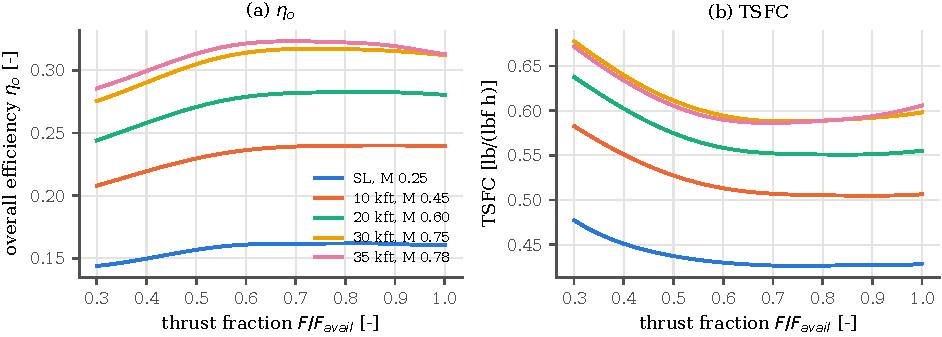
\includegraphics[width=\textwidth]{tf_maps.pdf}
\caption{Turbofan surrogate: (a) overall efficiency and (b) TSFC versus thrust fraction at five
flight conditions.}
\label{fig:tf-maps}
\end{figure}

\begin{table}[htbp]
\centering\small
\caption{Turbofan surrogate at the points printed by example 26 (nominal SLS thrust
\SI{240}{kN}).}\label{tab:tf-points}
\begin{tabular}{@{}lrrrrrr@{}}
\toprule
Condition & altitude [ft] & Mach & fraction & $\etao$ & TSFC [lb/(lbf\,h)] & $\lambda_T$ \\
\midrule
take-off & 0 & 0.25 & 1.00 & 0.160 & 0.429 & 0.770 \\
climb & \num{10000} & 0.55 & 0.90 & 0.269 & 0.552 & 0.524 \\
cruise & \num{35000} & 0.78 & 0.70 & 0.323 & 0.586 & 0.275 \\
fast cruise & \num{35000} & 0.85 & 0.85 & 0.335 & 0.618 & 0.275 \\
descent & \num{20000} & 0.60 & 0.30 & 0.244 & 0.638 & 0.422 \\
\bottomrule
\end{tabular}
\end{table}

Figure~\ref{fig:tf-lapse}(b) shows the fitted thrust lapse and the deck points.
\code{Powertrain.ThrustLapse} returns the map value when a turbofan model is attached, and
otherwise the Mattingly high-bypass form $\delta\,(1 - 0.49\sqrt{M})$~\cite{mattingly}. The two
differ widely at altitude: at \SI{35000}{ft} and Mach 0.78 the map gives 0.275 and the fallback
0.133; at sea level and Mach 0.25 they give 0.770 and 0.755. The fallback is therefore only a
placeholder. Above the box the inputs are clipped: the lapse at \SI{39000}{ft} and Mach 0.80 is
0.273, the value at \SI{35000}{ft}. A ceiling requirement above \SI{35000}{ft} is therefore
optimistic on available thrust, as \code{HBTF_turbofan.py} and
\code{validation/a320_reference.md} state.

\begin{figure}[htbp]
\centering
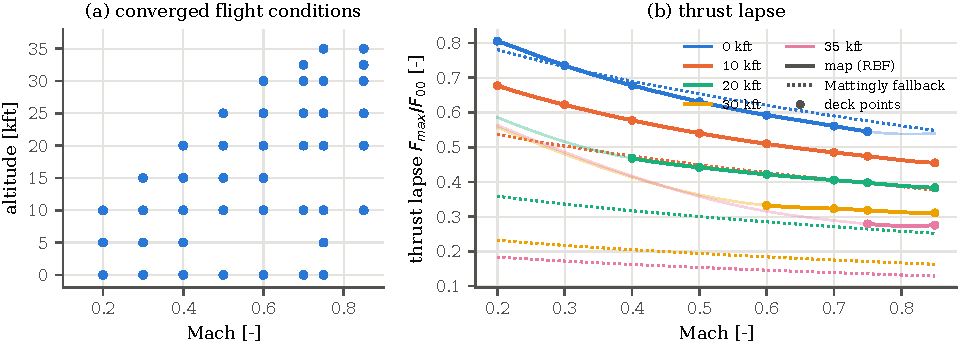
\includegraphics[width=\textwidth]{tf_lapse.pdf}
\caption{(a) Flight conditions of the turbofan deck. (b) Full-throttle thrust lapse: RBF (solid
where the deck has points at that altitude, faint elsewhere), deck points, and the Mattingly
fallback (dotted).}
\label{fig:tf-lapse}
\end{figure}

\subsection{Thrust-rated sizing}\label{sec:tf-sizing}
A turbofan is rated on thrust. \code{Performance.PoWTO} returns the thrust power per unit mass,
$(DV + W\,\mathrm{ROC})/m$, with no propulsive efficiency in it. Hence $T/W = (P/W)/(gV)$. The
constraint diagram divides every requirement by \code{Powertrain.SizingDenominator}, which is
the power lapse for every power-rated configuration and
\begin{equation}
  \texttt{SizingDenominator} = g\,V\,\lambda_T(h, M)
\end{equation}
for a turbofan. The design point \code{DesignPW} is then a dimensionless sea-level
thrust-to-weight ratio, exposed as \code{results().DesignTW}. Because each requirement has its
own speed, the minimum-thrust point and the minimum-power point are different points.

In the powertrain graph the turbofan is one node with efficiency $\etao$ and unit gearbox and
fan efficiencies. Therefore \code{PRatio[0]} $= 1/\etao$, and the fuel closure
$\dot m_f = P_p/(\etao\,E_f)$ is exactly the TSFC closure of~\eqref{eq:etao} when
$E_f$ equals the LHV of the map, as in \code{turbofan_config} ($E_f = \SI{43.0}{MJ/kg}$). The
mission and weight paths are those of the conventional configuration.

\code{WeightPowertrain} sizes the engine on the largest of three sea-level thrusts: the mission
peak thrust divided by the lapse at its altitude and Mach, the take-off or OEI thrust divided by
the lapse at the take-off altitude, and the constraint-diagram thrust
$\texttt{DesignPW}\cdot W_{TO}\,g$. The engine mass is that thrust over $g$ and the installed
thrust-to-weight \code{engine_thrust_to_weight} (default 5.5). \code{engineRating} then carries a
thrust in newtons, and \code{results().engineRating_units} is \code{'N'}.
\code{report_turbofan_sizing} names the sizing case and compares it with the nominal: it warns
when the requirement exceeds the nominal, and when it is less than half of it.

On TF the design closes at $W_{TO} = \SI{79883}{kg}$, $T/W = 0.2536$, $W/S =
\SI{4590}{N/m^2}$ and a wing area of \SI{170.7}{m^2}. The three sizing cases are
\SI{240.1}{kN} (mission peak), \SI{198.7}{kN} (take-off/OEI) and \SI{198.7}{kN} (constraint
diagram). The mission peak sets the rating, which is 0.05\,\% below the nominal of
\SI{240.2}{kN}, so the map is read against a nominal that matches the sized engine and
\code{report_turbofan_sizing} does not warn. At the cruise constraint (\SI{10058}{m}, Mach
0.78) the thrust is \SI{46.4}{kN}, $\etao = 0.3230$ and TSFC $= \SI{0.593}{lb/(lbf\,h)}$; the
thrust-weighted mean TSFC over the mission is \SI{0.594}{lb/(lbf\,h)}.

\subsection{A320 validation}\label{sec:a320}
\code{trunk/validation/a320_reference.py} compares TF with the A320-200 (CFM56-5B4, weight
variant WV017). \code{a320_reference.md} records each reference value and labels it primary
(Airbus ACAP, EASA TCDS) or secondary. Table~\ref{tab:a320} gives four design points that we
computed with its functions, labelled as in its \code{main}: (A) the default minimum-thrust
point; (B) the landing-limited wing loading that PhlyGreen derives from its own landing
constraint (\SI{582.6}{kg/m^2}); (C) the same wing loading with the Class-I empty-weight
regression scaled so that the empty weight equals the reference OEW; and (E) the wing loading of
the real aircraft (\SI{636.2}{kg/m^2}).

\begin{table}[htbp]
\centering\small
\caption{TF against the A320-200 reference of \texttt{validation/a320\_reference.md}. Relative
differences in brackets. In case C the OEW is fitted, not predicted.}\label{tab:a320}
\setlength{\tabcolsep}{4pt}
\begin{tabular}{@{}lrrrrr@{}}
\toprule
Quantity & reference & A: min.\ thrust & B: landing & C: B, OEW fitted & E: ref.\ $W/S$ \\
\midrule
MTOW [kg] & \num{78000} & \num{79884} (+2.4\,\%) & \num{75653} ($-$3.0\,\%) & \num{77260} ($-$0.9\,\%) & \num{74812} ($-$4.1\,\%) \\
OEW [kg] & \num{42600} & \num{43194} (+1.4\,\%) & \num{41345} ($-$2.9\,\%) & \num{42600} (fitted) & \num{40975} ($-$3.8\,\%) \\
wing area [m$^2$] & 122.6 & 170.7 (+39.3\,\%) & 129.9 (+5.9\,\%) & 132.6 (+8.2\,\%) & 117.6 ($-$4.1\,\%) \\
SLS thrust [kN] & 240.2 & 240.1 ($-$0.05\,\%) & 227.4 ($-$5.3\,\%) & 232.4 ($-$3.2\,\%) & 226.5 ($-$5.7\,\%) \\
\bottomrule
\end{tabular}
\end{table}
MTOW and SLS thrust are primary values, OEW and wing area secondary. In case C, \code{calibrate_structure_to_oew} finds the
regression factor $k$ as the root of $\mathrm{OEW}(k) - \mathrm{OEW}_{ref}$: it raises $k$ from 1
in steps of 0.02 until the OEW passes the target, then refines it with Brent's method. Its
docstring explains why a plain update $k \leftarrow k\,\mathrm{OEW}_{ref}/\mathrm{OEW}$ is not
used: the converged OEW grows by more than 2\,\% per 1\,\% of $k$, so that update overshoots and
diverges. Our run gives $k = 1.013$.

The minimum-thrust point has a much larger wing than the real aircraft, because minimizing the
installed thrust is not the same as minimizing the take-off weight. At the landing-limited and
the reference wing loadings the masses are 3 to 4\,\% and the thrust 5 to 6\,\% below the
reference. With the empty weight fitted (C), MTOW is within 1\,\% and the thrust 3.2\,\% below
the reference, and the wing is 8.2\,\% larger. In every case the mission peak sets the thrust. The emission indices of the
turbofan are referenced to the CFM56-7B27E, not the -5B4 (Section~\ref{sec:em-tf}).

%% ======================================================================================
\section{Propeller}\label{sec:prop}
%% ======================================================================================

\subsection{Hamilton-Standard model}\label{sec:hamilton}
\code{propeller_hamilton.py:Propeller.ComputePropEfficiency(alt, V, P)} implements the
Hamilton-Standard generalized blade-element charts. The chart data and the interpolation
routines (\code{_unint}, a four-point cubic-like interpolation with slope continuity, and
\code{_biquad}) are in \code{propeller_hamilton_tables.py}. The geometry comes from
\code{aircraft.PropellerInput}: diameter $D$, rpm, number of blades $B$, activity factor AF and
integrated design lift coefficient $c_{l_i}$. The engine count is \code{powertrain.n_engines}, and
the shaft power passed to the model is the total of all propellers.

The model forms the advance ratio, the power coefficient and the tip Mach number (imperial
units, as in the code),
\begin{equation}
  J = \frac{\pi V}{V_{tip}}, \qquad
  C_P = \frac{P_{hp}\cdot 10\mathrm{e}10/(2\cdot 6966)}{\sigma\,V_{tip}^3\,D^2}, \qquad
  M_{tip} = \frac{V_{tip}}{a},
\end{equation}
with $V_{tip} = \pi D\,\mathrm{rpm}/60$ [ft/s], $P_{hp}$ the shaft power per engine and $\sigma$
the density ratio. It corrects $C_P$ for activity factor, blade number and $c_{l_i}$, reads the
blade angle and the thrust coefficient from the charts at the four tabulated advance ratios
around $J$, interpolates in $J$, and iterates the thrust coefficient so that its
$c_{l_i}$-corrected value matches the chart. A compressibility factor $X_{FT}$ applies when the
helical Mach number exceeds a critical value. The efficiency is
\begin{equation}
  \eta_P = \frac{J\,C_T\,X_{FT}}{C_P}.
\end{equation}
Odd blade numbers are interpolated between the even charts. Out-of-table look-ups are counted
and printed. \code{HamiltonPropellerEfficiency} clips the result to $[0.4, 1]$.

Figure~\ref{fig:prop}(a) shows the model with the geometry of
\code{examples/25_fuelcell_battery_class_ii_models.py}: $D = \SI{13}{ft}$, \SI{1063}{rpm}, two
engines, six blades, AF 167, $c_{l_i} = 0.5$. The tip speed is \SI{723.6}{ft/s} and the tip Mach
number 0.648 at sea level. The peak efficiency is 0.709 at \SI{1}{MW} (\SI{0.5}{MW} per engine)
and 0.841 at \SI{4}{MW} at sea level, and between 0.832 and 0.856 at \SI{6000}{m}. At low
loading and high advance ratio the efficiency falls to zero, where the thrust coefficient
iteration finds no positive thrust.

\paragraph{Design with the Hamilton propeller.} On TP with this geometry the design closes at
$W_{TO} = \SI{18984}{kg}$ and \SI{2380}{kg} of fuel, against \SI{17843}{kg} and \SI{1939}{kg}
with the constant 0.9. The propeller is read at its shaft input (Section~\ref{sec:interface}).
The fuel-weighted mean propeller efficiency is 0.815. It ranges from 0.854 to the clip value 0.4,
which 26 of the 229 mission points reach, all in descent at propulsive powers below
\SI{210}{kW}.

The component-power iteration converges at every accepted point of the mission. The design
emits 7 non-convergence warnings, all from trial evaluations of the mission integrator at
\SI{8000}{m} and \SI{90}{m/s}, with propulsive powers from 4.17 to \SI{4.24}{MW}. At that
condition the thrust power $P\,\eta_P(P)$ of the unclipped Hamilton model peaks at
\SI{4.234}{MW}, at a shaft power of about \SI{8.9}{MW}. A demand at or above the peak has no
solution on the model's own curve; the only one left is on the 0.4 floor of the wrapper, at a
much larger shaft power. The returned ratios at those trial points are those of the last pass.

\subsection{RBF propeller surrogate}\label{sec:prop-rbf}
\code{propeller_surrogate.py:PropellerSurrogate} is fitted from
\code{data/propeller_data_rbf.csv}: 1000 rows on a $10\times10\times10$ grid of altitude (0 to
\SI{10000}{m}), airspeed (10 to \SI{180}{m/s}) and power (50 to \SI{2500}{kW}), with the rpm and
pitch of a governed propeller and its efficiency. The generator
\code{data/PropellerGenerationCSV.py} imports a \code{PropellerSystem} class from a module
\code{Propeller_System} that is not in the repository, with $D = \SI{3.93}{m}$, six blades,
AF 120, $c_{l_i} = 0.5$ and two engines. The physical model behind the CSV therefore cannot be
inspected or rerun. The column \code{EM_Power_kW} holds watts; the loader detects this (mean
above \num{10000}) and divides by 1000. Eight rows have zero rpm, pitch and efficiency and are
kept in the fit. The rpm follows a schedule: 616 rows lie near \SI{1000}{rpm} (high speed) and
305 near \SI{1200}{rpm} (low speed).

The class normalizes each input to $[0, 1]$ with the data range, clipping outside it, and fits
two RBFs with the \code{multiquadric} kernel and a smoothing of 0.1: a pitch governor
$\beta(P, h, V, \mathrm{rpm})$ and an efficiency map $\eta(P, h, V, \beta, \mathrm{rpm})$. The fit
runs each time the object is built (\SI{0.13}{s} in our run); there is no pickle. At the 992 rows with
non-zero rpm the efficiency map errs by an rms of 0.041 and at most 0.319; the governor errs by
an rms of \SI{0.087}{\degree}.

\code{PropellerSurrogateEfficiency.eta(op)} divides the power by \code{n_engines}, converts it to
kW, solves the governor at the rpm of \code{propeller_rpm} (default 1200) and
evaluates the map. Figure~\ref{fig:prop}(b) shows one slice of the data (\SI{5556}{m},
\SI{867}{kW}) with the map at the rows' own pitch and rpm, and the governor-plus-map chain at
1000 and \SI{1200}{rpm}. On TP (two engines) the design closes at $W_{TO} = \SI{19962}{kg}$
with \SI{2790}{kg} of fuel. The fuel-weighted mean efficiency is 0.780, and the minimum 0.266,
in descent at low power. The component-power iteration converges everywhere: the design emits
no non-convergence warning. The rpm is \code{EnergyConfig.propeller_rpm} (legacy key
\texttt{Propeller RPM}), with a default of \SI{1200}{rpm}.

\begin{figure}[htbp]
\centering
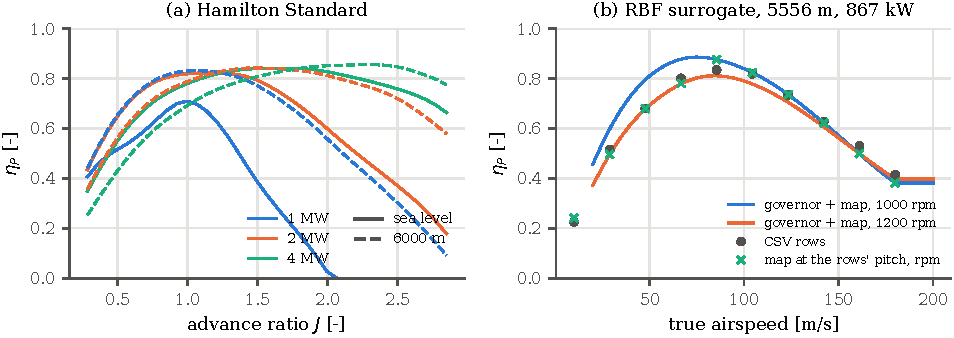
\includegraphics[width=\textwidth]{propeller.pdf}
\caption{(a) Hamilton-Standard efficiency versus advance ratio for the example-25 geometry at
three total shaft powers, at sea level and at \SI{6000}{m}. (b) RBF propeller surrogate at one
slice of its data.}
\label{fig:prop}
\end{figure}

%% ======================================================================================
\section{Emission indices: the physical pipeline}\label{sec:em-physics}
%% ======================================================================================

\subsection{Overview}
An emission index $\EI{X}$ is the mass of species X emitted per kilogram of fuel burnt [g/kg].
PhlyGreen computes the NO$_x$, CO and UHC indices offline in two stages,
\[
  (h, M, \mathrm{PC}) \xrightarrow{\ \text{pyCycle deck}\ } (T_3, p_3, \mathrm{FAR}, \dot m_{3})
  \xrightarrow{\ \text{Cantera CRN}\ } (\EI{NO_x}, \EI{CO}, \EI{UHC}),
\]
where PC is the power or thrust fraction, and $T_3$, $p_3$, FAR and $\dot m_3$ are the
temperature, pressure, fuel-to-air ratio and air flow at the combustor inlet. The deck is engine
specific. The CRN is the same code for both engines, with engine-specific calibration constants.
The pipeline lives in \code{emissions_pipeline/}; its notes (\code{README.md} and
\code{EMISSIONS_MODEL_NOTES.md}) record the provenance: the CRN comes from A.~Pietrosanto's
thesis~\cite{pietrosanto} and was calibrated to ICAO LTO data of the CFM56. Soot is not modelled
by this pipeline; a separate soot CRN (\code{crn_soot/}, from F.~Bassis's thesis~\cite{bassis}) is
kept for a future extension and is not used.

\subsection{The chemical reactor network}\label{sec:crn}
\code{crn/evap_model_ottimizzato.py:run_crn_evap_mode(key, params)} builds and integrates a
three-stage network for one combustor state:
\begin{itemize}
\item \textbf{Primary zone (PZ).} Nine perfectly stirred reactors in parallel. The primary-zone
  air ($\mathrm{ARPZ} = 30.82\,\%$ of the core air) is split with Gaussian weights over nine
  equivalence ratios centred on $\phi_{PZ} = \mathrm{FAR}/(\mathrm{FAR}_{st}\,\mathrm{ARPZ})$
  with a standard deviation of $0.15\,\phi_{PZ}$, to represent unmixedness. Eight reactors
  receive vaporized fuel; the ninth receives the fuel recovered from the liquid phase.
\item \textbf{Secondary zone (SZ).} One reactor fed by the mixed PZ products and 23.02\,\% of
  the air.
\item \textbf{Dilution zone (DZ).} One reactor fed by the SZ products and 46.15\,\% of the air,
  discharging to a back pressure $p_3\,(\Delta p/p)$.
\end{itemize}
The volumes follow a reference area of \SI{0.160}{m^2}, a length of \SI{0.178}{m} and zone
length fractions of 0.2029 (PZ), 0.1979 (SZ) and the rest (DZ). Each reactor starts from
nitrogen at \SI{1800}{K}, its inflows ramp up exponentially, and it is integrated until its
temperature and pressure settle. A reactor is declared steady after 60 consecutive steps with
relative changes of temperature and pressure below $10^{-7}$. For the secondary and dilution zones
these steps are counted only after five residence times of the zone (\code{N_TAU_MIN_STAGE}).
The docstring of \code{integrate_stage_stepwise} explains why: the first integrator steps of a
new reactor, of order $10^{-12}$~s, change the temperature by less than the tolerance, so
without that minimum time a zone could be returned at its unreacted inlet state.

The fuel is a three-component kerosene surrogate ($n$-decane 0.74, propylbenzene 0.15,
propylcyclohexane 0.11 by mole) with the Luche mechanism of \code{kerosene_surrogate_luche.yaml}
(92 species, 991 reactions). An evaporation model decides how much fuel reaches the PZ as vapour.
A Lefebvre-type correlation gives the Sauter mean diameter, a droplet law gives the evaporation
time $\tau_{evp}$, and the vaporized fraction is
\begin{equation}
  f_{vap} = 1 - \exp\!\left(-\frac{\tau_{mix}}{\tau_{evp}}\right), \qquad
  \tau_{mix} = 0.6\,\chi\,\tau_{res,PZ},
\end{equation}
with $\chi$ the mixer scale, a calibration constant of each mode. Of the liquid fraction,
5\,\% becomes soot (not tracked further), a temperature-dependent part vaporizes into the ninth
reactor, and the rest leaves as unburned hydrocarbons that never react (a bypass tracer).

The indices are computed from the DZ outlet: $\EI{NO_x}$ from the NO and NO$_2$ mass fractions,
$\EI{CO}$ from CO, and $\EI{UHC}$ as the gaseous hydrocarbons plus the bypass tracer, all
divided by FAR and expressed in g/kg. The function also returns a combustion efficiency
following Villette's Eq.~(6), named in its docstring. Its inputs are $T_3$, $p_3$, $\dot m_3$,
FAR, $\Delta p/p$ and $\chi$.

\subsection{Native calibration: CFM56-7B27E}\label{sec:crn-native}
The CRN carries the four ICAO LTO states of the CFM56-7B27E in \code{MODE_DATA}, with a mixer
scale for each: idle (7\,\%, \SI{477}{K}, \SI{3.78}{bar}, FAR 0.014, $\chi = 1.50$), approach
(30\,\%, \SI{619}{K}, \SI{10.75}{bar}, FAR 0.016, $\chi = 1.272$), climb (85\,\%, \SI{759}{K},
\SI{24.80}{bar}, FAR 0.024, $\chi = 1.071$) and take-off (100\,\%, \SI{795}{K},
\SI{28.80}{bar}, FAR 0.026, $\chi = 1.0$). The ICAO emission indices are written in the same
file. \code{scripts/check_crn.py} runs the CRN at these four states with its native air split.
Table~\ref{tab:crn-native} and Figure~\ref{fig:em-crn}(a,b) give the result.

\begin{table}[htbp]
\centering\small
\caption{CRN at its own four CFM56-7B27E LTO states against the ICAO values in the CRN file
(Cantera 3.2.0).}\label{tab:crn-native}
\begin{tabular}{@{}lrrrrrrr@{}}
\toprule
 & \multicolumn{3}{c}{$\EI{NO_x}$ [g/kg]} & \multicolumn{2}{c}{$\EI{CO}$ [g/kg]} & \multicolumn{2}{c}{$\EI{UHC}$ [g/kg]} \\
\cmidrule(lr){2-4}\cmidrule(lr){5-6}\cmidrule(l){7-8}
Mode & CRN & ICAO & diff. & CRN & ICAO & CRN & ICAO \\
\midrule
idle & 1.86 & 4.36 & $-$57\,\% & 36.06 & 29.39 & 1.06 & 1.54 \\
approach & 10.78 & 9.09 & +19\,\% & 6.90 & 2.82 & 0.11 & 0.05 \\
climb & 23.06 & 17.89 & +29\,\% & 1.62 & 0.17 & 0.022 & 0.02 \\
take-off & 27.66 & 23.94 & +16\,\% & 1.47 & 0.31 & 0.021 & 0.03 \\
\bottomrule
\end{tabular}
\end{table}

The CRN over-predicts NO$_x$ by 16 to 29\,\% at approach, climb and take-off, which reproduces
the figures quoted in \code{emissions_pipeline/README.md} and \code{docs/user-guide/emissions.md}.
At idle it under-predicts NO$_x$ by 57\,\%. CO is close at idle and five to ten times too high at
climb and take-off, where the certified values are below \SI{0.4}{g/kg}.

\begin{figure}[htbp]
\centering
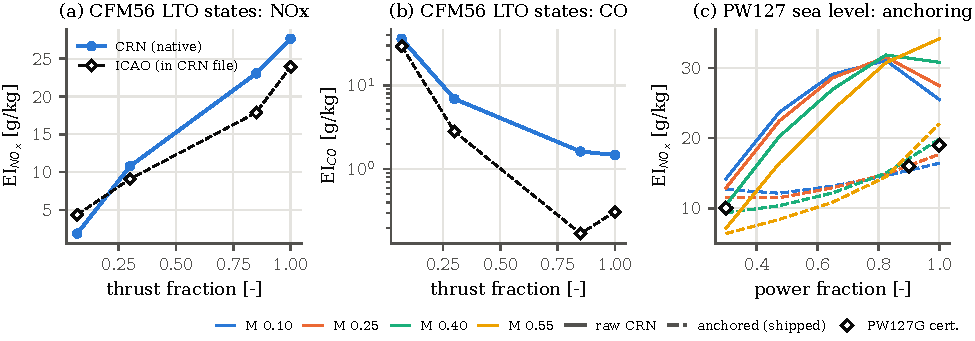
\includegraphics[width=\textwidth]{em_crn.pdf}
\caption{(a, b) CRN at the four CFM56-7B27E LTO states against ICAO. (c) PW127 sea-level slice:
raw CRN NO$_x$ (re-run by \texttt{check\_crn.py}), the anchored NO$_x$ of the shipped map, and
the certification NO$_x$ used for the anchor.}
\label{fig:em-crn}
\end{figure}

\subsection{PW127 chain and the certification anchor}\label{sec:em-pw127}
The turboprop chain has three scripts.
\begin{enumerate}
\item \code{pw127_deck.py} reuses the turboshaft classes of \code{Single_spool_GT.py} with an
  overall pressure ratio of 14.7 and a turbine inlet temperature of \SI{2370}{\degree R}. It
  bisects the rated power so that the sea-level-static fuel flow matches the take-off fuel flow
  of the certification data, \SI{0.16}{kg/s}.
\item \code{pw127_partpower.py} calibrates a gas-generator power schedule $G(f)$ so that the deck
  reproduces the certified fuel flow at the four LTO useful-power fractions (0.07, 0.30, 0.90,
  1.00), with a take-off gross power of \SI{3290}{hp}. The schedule stored in
  \code{_schedule.npy} gives 508, \num{1450}, \num{2854} and \SI{3287}{hp} at these fractions.
  The script then runs the deck at $G(f)\,\delta(h)$ over 5 altitudes (0 to \SI{30000}{ft})
  $\times$ 4 Mach numbers (0.10 to 0.55) $\times$ 5 fractions (0.3 to 1.0) and writes the 100
  combustor states of \code{pw127_crn_inputs_corrected.csv}. Mach 0 is excluded.
\item \code{build_pw127_surrogate.py} runs the CRN over these states and writes
  \code{data/PW127_Emission_Map.csv}, then calls \code{train_emission_surrogate.py}.
\end{enumerate}
The map coordinate of the PW127 artifact is therefore the fraction $f$ of a rated power lapsed by
the ISA pressure ratio: the deck runs at a gross power $G(f)\,\delta(h)$, as the turboshaft map
of Section~\ref{sec:gt-deck} runs at $f\,P_{des}\,\delta(h)$. \code{pw127_deck._od_state}
accepts a deck state only if the delivered shaft power is within 0.1\,\% of the request. A state
that fails from the fixed initial guesses is re-solved warm-started from a converged neighbour,
whose full model state is restored, and then by a power continuation; a state that still fails
stops the script. Every point of the $G(f)$ calibration curve passes the same test. All 100
envelope states are converged, and none of them has the fuel-to-air ratio of the initial guess,
0.017.

The certification data are the PW127G entry of the FOCA/EASA emission-factor database (source
EASA 2024), transcribed in \code{EMISSIONS_MODEL_NOTES.md} (Table~\ref{tab:pw127-cert}). The
database itself is not in the repository.

\begin{table}[htbp]
\centering\small
\caption{PW127G LTO data as transcribed in \texttt{EMISSIONS\_MODEL\_NOTES.md}, Section 3a. The
NO$_x$ anchor of \texttt{build\_pw127\_surrogate.py} uses the approach, climb and take-off NO$_x$
at power fractions 0.30, 0.90 and 1.00.}\label{tab:pw127-cert}
\begin{tabular}{@{}lrrrr@{}}
\toprule
Mode & fuel flow [kg/s] & $\EI{NO_x}$ [g/kg] & $\EI{CO}$ [g/kg] & $\EI{UHC}$ [g/kg] \\
\midrule
taxi/idle & 0.04 & 5.0 & 20.0 & 0.0 \\
approach & 0.08 & 10.0 & 4.0 & 0.0 \\
climb & 0.14 & 16.0 & 2.0 & 0.0 \\
take-off & 0.16 & 19.0 & 2.0 & 0.0 \\
\bottomrule
\end{tabular}
\end{table}

The CFM56 calibration does not fit the leaner PW127 combustor, so the build script patches the
CRN when it imports it:
\begin{itemize}
\item the primary-zone air fraction becomes $\mathrm{ARPZ} = 0.24$, and the SZ and DZ fractions
  are rescaled to keep the sum at one (\code{calibrate_crn_pw127.py} scans ARPZ against the four
  certified modes);
\item the mixer scale is interpolated in $T_3$ between the four CFM56 modes and floored at 1.20;
\item the pressure-loss factor is fixed at 0.95.
\end{itemize}
With these patches the notes report that the CRN matches the certified CO, but that its NO$_x$
rises with power too steeply for the flat certified curve. The NO$_x$ is therefore
\emph{certification-anchored}: it keeps the altitude, Mach and power trend of the CRN and is
rescaled to the certified level at sea level,
\begin{equation}
  \EI{NO_x}(h, M, \mathrm{PC}) = \EI{NO_x}^{CRN}(h, M, \mathrm{PC})\;
  \frac{\EI{NO_x}^{cert}(\mathrm{PC})}{\overline{\EI{NO_x}^{CRN}}(0, \mathrm{PC})},
  \label{eq:anchor}
\end{equation}
where $\EI{NO_x}^{cert}$ is a monotone (PCHIP) interpolation of 10, 16 and \SI{19}{g/kg} at
fractions 0.30, 0.90 and 1.00, and the denominator is the Mach average of the raw CRN at sea
level. The anchor is applied to every altitude. CO and UHC come from the CRN without rescaling.

\code{check_crn.py} re-runs the patched CRN on the 20 sea-level states. CO and UHC reproduce the
shipped map to a relative $4\times10^{-13}$, so the Cantera result is reproducible. The raw
NO$_x$ ranges from 7.2 to \SI{34.2}{g/kg}, against 6.4 to \SI{22.0}{g/kg} after anchoring
(Figure~\ref{fig:em-crn}(c)). At full power the raw CRN gives 25.5 to \SI{34.2}{g/kg}, so the
anchor divides it by 1.55 on average. The anchor makes the Mach average at sea level equal to
the certified value; individual Mach numbers keep the CRN spread (16.4 to \SI{22.0}{g/kg} at full
power). The UHC has no certification target, because the database gives zero at every mode.
At sea level and a fraction of 0.3 the CO is 4.2 to \SI{4.4}{g/kg} at the four Mach numbers.

\subsection{Turbofan chain}\label{sec:em-tf}
\code{build_turbofan_surrogate.py} takes the combustor state directly from the turbofan map
(Section~\ref{sec:tf-deck}), which exports $T_3$, $p_3$, FAR and the core air flow at the
combustor inlet for its 207 points. It runs the CRN with its native CFM56 calibration and
removes the three PW127 patches: no ARPZ change, no floor on the mixer scale, and the burner
pressure loss of the deck ($\Delta p/p = 0.946$). The NO$_x$ is not anchored. A command-line flag
\code{--anchor-nox} anchors it to the CFM56 ICAO values instead; the shipped artifact was built
without it.

The turbofan box ($T_3$ from 551 to \SI{769}{K}, FAR 0.0153 to 0.0250, core air flow 9.9 to
\SI{42.6}{kg/s}) lies inside the CRN calibration box in $T_3$ (477 to \SI{795}{K}) and close to it
in FAR (0.014 to 0.026). The mixer scale is interpolated in $T_3$ between the four CFM56 modes
and clipped at the end values.

The shipped map follows smooth trends. At the 126 points with a thrust fraction of 0.8 or more,
$\EI{CO}$ lies between 1.4 and \SI{4.7}{g/kg}; the sea-level points at these fractions give 1.4 to
\SI{2.3}{g/kg}, and the value rises with altitude. The largest CO of the map, \SI{14.4}{g/kg}, is
at a fraction of 0.3 (\SI{30000}{ft}, Mach 0.6). In the PW127 map the four high-power points with
CO above \SI{10}{g/kg} are at \SI{30000}{ft} and a fraction of 0.825, where the whole column is
high.

%% ======================================================================================
\section{Emission-index surrogates}\label{sec:em-surrogate}
%% ======================================================================================

\subsection{Artifact format and run time}
\code{train_emission_surrogate.py} fits one RBF per species over (altitude [ft], Mach, PC), each
with its own \code{StandardScaler}, the \code{multiquadric} kernel and a smoothing of 0.1.
$\EI{CO}$ and $\EI{UHC}$, which span decades, are fitted to $\log_{10}$ of the value. The pickle
is a plain dictionary: \code{inputs}, \code{outputs}, \code{tag}, \code{input_ranges} and, per
output, \code{kind} (\code{'rbf'}), \code{scaler}, \code{model} and \code{log}. Two artifacts
ship (Table~\ref{tab:em-artifacts}).

\begin{table}[htbp]
\centering\small
\caption{The two emission-index artifacts.}\label{tab:em-artifacts}
\begin{tabularx}{\textwidth}{@{}lXX@{}}
\toprule
 & \code{Emission_Model_PW127.pkl} & \code{Emission_Model_Turbofan.pkl} \\
\midrule
data & \code{PW127_Emission_Map.csv}, 100 points & \code{Turbofan_Emission_Map.csv}, 207 points \\
third coordinate PC & shaft power over rated power lapsed by $\delta(h)$ & thrust over full-throttle thrust, $F/F_{max}(h, M)$ \\
box & 0--\SI{30000}{ft}, Mach 0.10--0.55, PC 0.3--1.0 & 0--\SI{35000}{ft}, Mach 0.20--0.85, PC 0.3--1.0 \\
combustor & CFM56 CRN patched to PW127 & CFM56 CRN, native \\
NO$_x$ & anchored to PW127G certification & raw CRN \\
range of $\EI{NO_x}$ & 1.0--\SI{22.0}{g/kg} & 6.1--\SI{28.0}{g/kg} \\
range of $\EI{CO}$ & 2.3--\SI{23.8}{g/kg} & 1.4--\SI{14.4}{g/kg} \\
range of $\EI{UHC}$ & 0.0002--\SI{1.14}{g/kg} & 0.015--\SI{0.157}{g/kg} \\
selected for & \code{'Traditional'}, \code{'Hybrid'} (and any other) & \code{'Turbofan'} \\
\bottomrule
\end{tabularx}
\end{table}

\code{EmissionSurrogate(model_path)} loads an artifact and \code{predict(X)} returns a
dictionary of arrays for inputs in the order of \code{inputs}, clipped to the box.
\code{predict_op(alt_ft, mach, pc)} returns floats for one point. \code{default_model_path(configuration)}
returns the turbofan artifact for \code{'Turbofan'} and the PW127 artifact otherwise. A missing
file raises \code{FileNotFoundError}. The surrogate does not form the third coordinate itself:
the caller must pass the quantity the map was generated at (Table~\ref{tab:em-artifacts}).
\code{ClimateImpact._surrogate_load_fraction} does it for the mission (Section~\ref{sec:em-path}).

\subsection{Accuracy}
Table~\ref{tab:em-fit} gives the relative errors at the training points and in leave-one-out
(refit without the point, in memory, with the settings of the trainer). The smoothing of 0.1
makes the surrogate a regression, not an interpolant.

\begin{table}[htbp]
\centering\small
\caption{Relative errors of the emission surrogates (mean absolute / rms / maximum).}\label{tab:em-fit}
\begin{tabular}{@{}llll@{}}
\toprule
Artifact, species & at training points & leave-one-out \\
\midrule
PW127, NO$_x$ & 1.1 / 1.5 / 5.5\,\% & 4.0 / 6.0 / 23\,\% \\
PW127, CO & 0.6 / 0.8 / 4.1\,\% & 2.2 / 3.8 / 23\,\% \\
PW127, UHC & 1.8 / 2.3 / 7.6\,\% & 6.5 / 9.5 / 37\,\% \\
Turbofan, NO$_x$ & 0.3 / 0.5 / 3.8\,\% & 0.8 / 1.8 / 16\,\% \\
Turbofan, CO & 0.2 / 0.3 / 1.4\,\% & 0.6 / 0.9 / 4.4\,\% \\
Turbofan, UHC & 6.4 / 11 / 57\,\% & 13 / 23 / 110\,\% \\
\bottomrule
\end{tabular}
\end{table}

Both surrogates follow their NO$_x$ and CO data closely. The leave-one-out rms is 6.0\,\% (PW127)
and 1.8\,\% (turbofan) on NO$_x$, and 3.8\,\% and 0.9\,\% on CO. The largest leave-one-out errors
sit at the edges of the box. For the PW127 NO$_x$ it is +23\,\% at \SI{30000}{ft}, Mach 0.1 and a
fraction of 0.3, where the anchored index is only \SI{2.0}{g/kg}; seven of the 100 points exceed
10\,\%. For the turbofan NO$_x$ it is +16\,\% at sea level, Mach 0.2 and a fraction of 0.3, the
only point above 10\,\%. The turbofan UHC is the least accurate quantity: its leave-one-out rms
is 23\,\%, 71 of the 207 points exceed 10\,\%, and the largest error is +110\,\% at
\SI{30000}{ft}, Mach 0.85 and a fraction of 0.9. Its values are small (0.015 to
\SI{0.157}{g/kg}), so the error is small in mass. At the training points the largest NO$_x$
residuals are below \SI{0.35}{g/kg} for both artifacts. \code{tests/regression/test_emission_surrogate.py}
checks the fit of the turbofan artifact with a log-space correlation above 0.9 and a median
relative error below 10\,\% for each species, and the PW127 artifact with a linear correlation
above 0.9 for NO$_x$ and CO; both pass.

\subsection{Maps and certification points}
Figures~\ref{fig:em-maps-pw127} and~\ref{fig:em-maps-tf} show the three indices versus the
fraction at several altitudes, with the sea-level data and the certification points.

\begin{figure}[htbp]
\centering
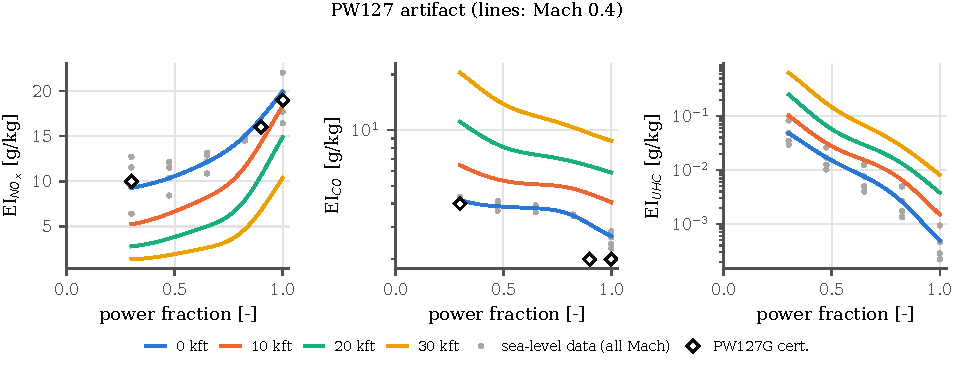
\includegraphics[width=\textwidth]{em_maps_pw127.pdf}
\caption{PW127 emission surrogate versus power fraction at Mach 0.4 and four altitudes, with the
sea-level training data at every Mach number and the PW127G certification points
(Table~\ref{tab:pw127-cert}; UHC is zero and not shown).}
\label{fig:em-maps-pw127}
\end{figure}

\begin{figure}[htbp]
\centering
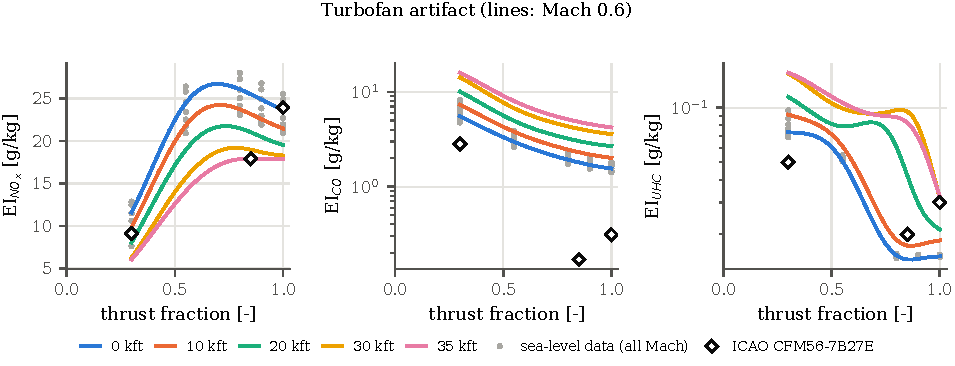
\includegraphics[width=\textwidth]{em_maps_tf.pdf}
\caption{Turbofan emission surrogate versus thrust fraction at Mach 0.6 and five altitudes, with
the sea-level training data and the CFM56-7B27E ICAO points.}
\label{fig:em-maps-tf}
\end{figure}

For the PW127 artifact, along the lines of Figure~\ref{fig:em-maps-pw127}, NO$_x$ rises with
power and CO and UHC fall with power at every altitude. For the turbofan artifact at Mach 0.6,
CO falls with thrust everywhere, while NO$_x$ peaks at a fraction between 0.70 (sea level) and
0.85 (\SI{35000}{ft}) and UHC has a shallow minimum near a fraction of 0.9 at sea level and \SI{10000}{ft}. In both maps
NO$_x$ falls and CO rises with altitude. At full thrust and Mach 0.75, for example, the turbofan data give a
NO$_x$ of 25.6 at sea level and \SI{18.3}{g/kg} at \SI{35000}{ft}, and a CO of 1.4 and
\SI{3.9}{g/kg}. Table~\ref{tab:em-cert} compares both artifacts at sea level with the
certification data, averaged over the Mach numbers of the sea-level grid. The PW127 NO$_x$
matches the anchor by construction. Its CO is 1.1 to 1.5 times the certified value at the three
flight modes. The turbofan NO$_x$ is 16\,\% high at approach, 38\,\% high at climb and 4\,\% low
at take-off. It is not monotone in thrust: the sea-level data peak at a fraction of 0.8 (mean
\SI{25.3}{g/kg} over Mach, up to \SI{28.0}{g/kg} at Mach 0.75, the largest value of the map) and
fall to a mean of \SI{23.0}{g/kg} at full thrust. The turbofan CO is 5 to 11 times the ICAO
value at climb and take-off, which follows from the native CRN at its own LTO states
(Table~\ref{tab:crn-native}).

\begin{table}[htbp]
\centering\small
\caption{Surrogates at sea level (mean over the Mach numbers of the sea-level grid: 0.10--0.55
for PW127, 0.20--0.75 for the turbofan) against the certification values written in the
repository.}\label{tab:em-cert}
\begin{tabular}{@{}llrrrrrr@{}}
\toprule
 & & \multicolumn{2}{c}{$\EI{NO_x}$ [g/kg]} & \multicolumn{2}{c}{$\EI{CO}$ [g/kg]} & \multicolumn{2}{c}{$\EI{UHC}$ [g/kg]} \\
\cmidrule(lr){3-4}\cmidrule(lr){5-6}\cmidrule(l){7-8}
Artifact & PC & surr. & cert. & surr. & cert. & surr. & cert. \\
\midrule
PW127 & 0.30 & 9.95 & 10.0 & 4.29 & 4.0 & 0.048 & 0.0 \\
 & 0.90 & 16.47 & 16.0 & 3.03 & 2.0 & 0.0013 & 0.0 \\
 & 1.00 & 19.03 & 19.0 & 2.60 & 2.0 & 0.0005 & 0.0 \\
Turbofan & 0.30 & 10.58 & 9.09 & 6.26 & 2.82 & 0.079 & 0.05 \\
 & 0.85 & 24.73 & 17.89 & 1.89 & 0.17 & 0.015 & 0.02 \\
 & 1.00 & 23.02 & 23.94 & 1.63 & 0.31 & 0.015 & 0.03 \\
\bottomrule
\end{tabular}
\end{table}

\subsection{Why the two artifacts are not interchangeable}
The two artifacts differ in three ways. First, the combustor: the PW127 map comes from a CRN
re-tuned to a lean turboprop combustor (richer primary zone, mixer floor) and anchored to its
certification NO$_x$; the turbofan map comes from the native CFM56 calibration. Second, the
coordinate: the PW127 map is keyed on the shaft-power fraction of a lapsed rating, in a deck
whose part-power schedule was calibrated to PW127 fuel flows; the turbofan map on the thrust
fraction of the HBTF deck. A fraction of 0.8 is a different combustor state in each. Third, the envelope: the
turboprop box stops at Mach 0.55 and \SI{30000}{ft}, the turbofan box starts at Mach 0.2. A
query outside a box is clipped to its edge, so a turbofan cruise read on the PW127 map would
return the Mach-0.55 value. \code{default_model_path} enforces the pairing by configuration, and
a test checks it.

%% ======================================================================================
\section{Emissions in the climate module}\label{sec:em-climate}
%% ======================================================================================

\code{ClimateImpact.calculate_mission_emissions} computes the mission emissions in kilograms.
CO$_2$, H$_2$O, SO$_4$ and soot are fixed indices times the burnt fuel \code{weight.Wf}, which
includes the ground segments. NO$_x$ follows \code{ClimateImpactConfig.einox_model}:
\code{'Filippone'} or \code{'Surrogate'}. With \code{'Surrogate'} the mission emissions also
contain CO and UHC. A fuel-cell configuration emits no NO$_x$, and \code{'Surrogate'} raises a
\code{ValueError} there.

Both NO$_x$ paths have two parts. The first walks the accepted points of the mission integrator
(\code{mission.integral_solution}), the flown mission and diversion. At each point it recovers the
propulsive power $P$ from \code{PoWTO}, calls the powertrain, and forms the fuel flow
$\dot m_f = P\,\texttt{PRatio[0]}/E_f$; it integrates $\EI{}\,\dot m_f$ with the trapezoidal
rule. This walk needs the continuous mission solution, \code{aircraft.MissionType = 'Continue'}.
\code{build_aircraft} sets it, and \code{ClimateImpact} assumes it when the attribute is
missing. The second part adds the ground segments: taxi-out, the take-off run and taxi-in
(\code{ClimateImpact._ground_legs}). Their fuel is in \code{weight.Wf} but not in the flown
mission. Each leg is taken at the duration and fuel flow that \code{Mission._ground_segments}
used (\code{mission._ground_fuel_legs_out} and \code{_in}), at the take-off condition, and at
\code{taxi_power_fraction} (default 7\,\%) or \code{takeoff_power_fraction} (default 1) of the
take-off propulsive power. The ground share is stored in \code{climateimpact.ground_emissions}.
NO$_x$, CO and UHC then cover the same fuel as CO$_2$.

\subsection{Filippone correlation}
The Filippone path uses a semi-empirical correlation~\cite{filippone} in the overall pressure
ratio OPR and the fuel flow per engine $\dot m_e$ [kg/s],
\begin{equation}
  \EI{NO_x} = 2\left(c_0 + c_1\,\mathrm{OPR} + c_2\,\mathrm{OPR}^2 + c_3\,\dot m_e + c_4\,\dot m_e^2
  + c_5\,\mathrm{OPR}\,\dot m_e\right),
\end{equation}
with three coefficient sets (\code{FILIPPONE_COEFF}: climb-out, idle, approach). On the flown
mission they are selected by breakpoints in the mission time: climb-out for the climbs, idle for
the cruises and approach for the descents. The breakpoints are found from the cruise altitudes
of the mission and diversion stages. On the ground the take-off run uses the climb-out set and
taxi the idle set. OPR is \code{EnergyConfig.opr} (default 15.77) and the engine count is
\code{powertrain.n_engines}. Figure~\ref{fig:em-filippone} shows the three branches, labelled
by the mission phase that uses them. The correlation knows neither altitude nor Mach number,
except through the phase and the fuel flow, and its value jumps at the phase boundaries.

\begin{figure}[htbp]
\centering
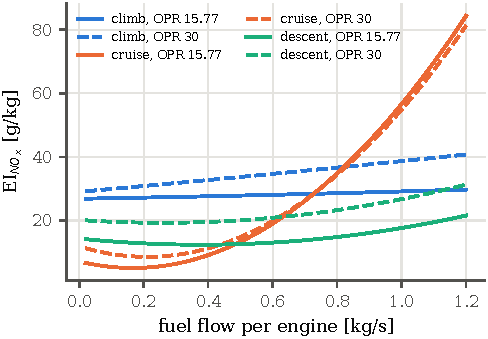
\includegraphics[width=0.6\textwidth]{em_filippone.pdf}
\caption{Filippone NO$_x$ index versus fuel flow per engine for the three coefficient sets
(climb-out, idle and approach, used in climb, cruise and descent), at OPR 15.77 (default) and 30
(\texttt{turbofan\_config}).}
\label{fig:em-filippone}
\end{figure}

\subsection{Surrogate path}\label{sec:em-path}
\code{_integrate_surrogate_emissions} loads the artifact of \code{default_model_path} (unless
\code{climateimpact.emission_surrogate} is set). At each mission point it forms the coordinates of
the map: altitude in feet, Mach number from the ISA temperature with the mission DISA, and the
load fraction of \code{_surrogate_load_fraction}. Each artifact is read at the coordinate it was
generated at:
\begin{itemize}
\item \textbf{Traditional and Hybrid (PW127 map)}: the gas-turbine shaft power over the rated
  power lapsed by the ISA pressure ratio,
  \begin{equation}
    \mathrm{PC} = \frac{\texttt{PRatio[1]}\,P}{\texttt{engineRating}\;\delta(h)} .
    \label{eq:pc-tp}
  \end{equation}
  This is the coordinate of \code{pw127_partpower.py}, which runs the deck at $G(f)\,\delta(h)$
  (Section~\ref{sec:em-pw127}). In a hybrid, \code{PRatio[1]} is the thermal share only: the
  battery share does not pass through the combustor.
\item \textbf{Turbofan}: the thrust $F = P/V$ over the lapsed available thrust,
  $\mathrm{PC} = F/(\texttt{engineRating}\cdot\lambda_T(h, M))$, the thrust fraction of the HBTF
  map.
\end{itemize}
Both \code{engineRating} and the fraction refer to the whole aircraft; the fraction is the same
per engine. Inputs outside the box of the map are clipped to its edge.

How~\eqref{eq:pc-tp} behaves depends on the rating lapse of Section~\ref{sec:gt-lapse}. With the
Class-II gas-turbine map, \code{engineRating} is rated with $\delta$ itself, so the fraction
reaches exactly 1 at the point that sets the rating and never exceeds it. With a constant
gas-turbine efficiency, the rating uses $(\rho/\rho_0)^{0.75}$, which falls more slowly than
$\delta$. At altitude the fraction then exceeds 1 and is clipped to the map edge, so the map is
read at its full-power indices.

The ground legs are read at the same coordinate, at the take-off altitude, with Mach 0 for taxi
and the take-off Mach number for the take-off run. Taxi at 7\,\% of the take-off power gives a
fraction of 0.04 to 0.06 on our designs, below the 0.3 edge of both maps. It is therefore read
at the edge, at approach-like indices: relative to an idle index the taxi NO$_x$ is
overestimated and the taxi CO underestimated, as the docstring of the method states.

To check the implementation, \code{compute_data.py} recomputes the coordinate and the
integral of the flown mission independently of \code{ClimateImpact}. Adding the ground share of
\code{ground_emissions}, it reproduces the NO$_x$, CO and UHC masses of \code{ClimateImpact} on
all three designs below to the printed digits.

\subsection{Mission results}\label{sec:em-mission}
Table~\ref{tab:em-mission} gives the mission emissions of TP (constant gas-turbine efficiency),
TP with the Class-II gas turbine (nominal from the rating, two engines) and TF, with both NO$_x$
models. Table~\ref{tab:em-fraction} summarizes the load fraction along each mission, and
Figure~\ref{fig:em-mission} shows the indices and the fractions.

\begin{table}[htbp]
\centering\small
\caption{Mission emissions [kg], flown mission and diversion plus ground segments. Mean index =
NO$_x$ mass over the burnt fuel $W_f$. The ground columns give the share of the ground
segments.}\label{tab:em-mission}
\setlength{\tabcolsep}{4pt}
\begin{tabular}{@{}lrrrrrrr@{}}
\toprule
Case & $W_f$ & NO$_x$ & mean $\EI{NO_x}$ [g/kg] & CO & UHC & ground fuel & ground NO$_x$ \\
\midrule
TP, Filippone & \num{1939.4} & 22.34 & 11.5 & -- & -- & 42.3 & 0.53 \\
TP, Surrogate & \num{1939.4} & 23.44 & 12.1 & 12.40 & 0.023 & 42.3 & 0.56 \\
TP Class II, Filippone & \num{1216.6} & 14.13 & 11.6 & -- & -- & 34.9 & 0.42 \\
TP Class II, Surrogate & \num{1216.6} & 6.80 & 5.6 & 9.72 & 0.059 & 34.9 & 0.43 \\
TF, Filippone (OPR 30) & \num{20939} & 287.6 & 13.7 & -- & -- & 200.5 & 3.37 \\
TF, Surrogate & \num{20939} & 372.0 & 17.8 & 112.5 & 1.95 & 200.5 & 2.25 \\
\bottomrule
\end{tabular}
\end{table}

\begin{table}[htbp]
\centering\small
\caption{Load fraction PC of the emission map along the flown mission: number of integrator
points, points above 1 (clipped to full power) and below 0.3 (clipped to 0.3), maximum, and
fuel-weighted mean per phase (phases of the Filippone breakpoints).}\label{tab:em-fraction}
\begin{tabular}{@{}lrrrrrrr@{}}
\toprule
Case & points & $>1$ & $<0.3$ & max & climb & cruise & descent \\
\midrule
TP & 239 & 132 & 29 & 1.75 & 1.14 & 0.88 & 0.20 \\
TP Class II & 232 & 0 & 38 & 1.00 & 0.63 & 0.46 & 0.16 \\
TF & 220 & 0 & 49 & 1.00 & 0.83 & 0.58 & 0.20 \\
\bottomrule
\end{tabular}
\end{table}

On TP with the constant gas-turbine efficiency the surrogate gives 5\,\% more NO$_x$ than the
Filippone correlation. The agreement in total hides different distributions. Weighted by fuel
over the phases of the Filippone breakpoints, Filippone gives \SI{27.0}{g/kg} in climb,
\SI{5.8}{g/kg} in cruise and \SI{14.1}{g/kg} in descent, while the surrogate gives 16.5, 10.1
and \SI{5.5}{g/kg}. The surrogate reads 132 of the 239 points above full power, up to a
fraction of 1.75, because of the rating lapse; it reads them at its full-power indices.

On TP with the Class-II gas turbine the surrogate gives 52\,\% less NO$_x$ than Filippone (mean
index 5.6 against \SI{11.6}{g/kg}). The engine is rated with $\delta$, so its sea-level rating
is \SI{5402}{kW} against \SI{3107}{kW} for the constant-efficiency design, and the same flight
reads the map at about half the fraction: 0.46 in cruise against 0.88. There the PW127 map gives
lower NO$_x$ and higher CO. The surrogate gives 9.8, 4.9 and \SI{4.9}{g/kg} over the three phases;
Filippone, which sees only the fuel flow and the phase, gives 27.0, 6.2 and \SI{14.1}{g/kg}, close
to its values on the constant-efficiency design. The CO is \SI{9.7}{kg}, against \SI{12.4}{kg}
on the constant-efficiency design, which burns 59\,\% more fuel.

On TF the surrogate gives 29\,\% more NO$_x$ than Filippone at OPR 30 (mean index 17.8 against
\SI{13.7}{g/kg}). Filippone gives \SI{36.6}{g/kg} in climb, \SI{11.0}{g/kg} in cruise and
\SI{19.4}{g/kg} in descent; the surrogate gives 22.0, 17.5 and \SI{9.1}{g/kg}. The turbofan CO
(\SI{112.5}{kg}) follows from a CO index that the native CRN over-predicts at high thrust
(Section~\ref{sec:crn-native}).

The ground segments burn \SI{42.3}{kg} of fuel on TP, \SI{34.9}{kg} on TP Class II and
\SI{200.5}{kg} on TF, and add 0.4 to \SI{0.6}{kg} of NO$_x$ on the turboprops and 2.3 to
\SI{3.4}{kg} on TF. The take-off run is read at a fraction of 0.87 (TP), 0.58 (TP Class II) and
0.54 (TF).

\begin{figure}[htbp]
\centering
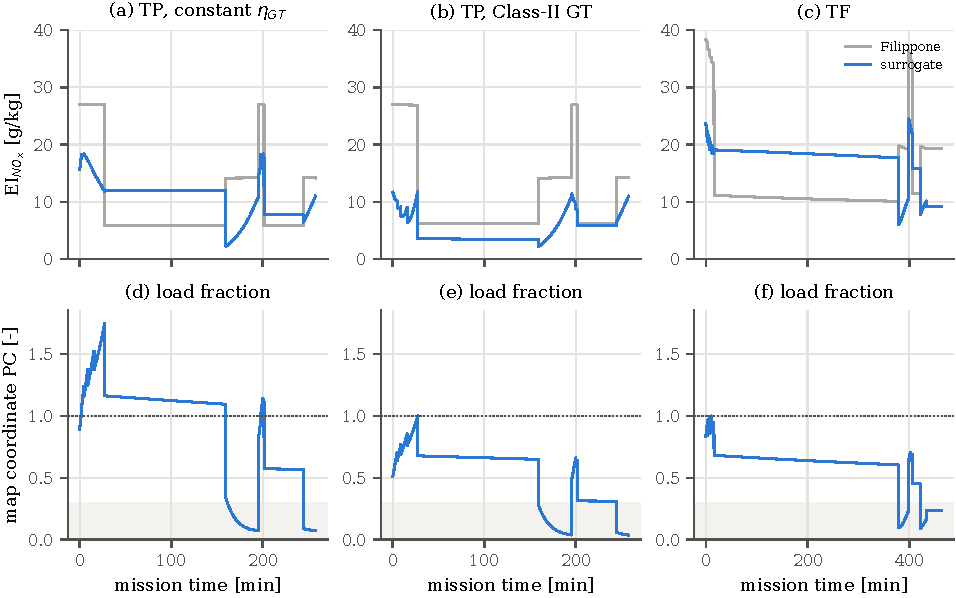
\includegraphics[width=\textwidth]{em_mission.pdf}
\caption{NO$_x$ index (top) and map coordinate PC (bottom) along the flown missions of TP
(constant $\eta_{GT}$), TP with the Class-II gas turbine, and TF. Grey band: below the training
range of the map (read at 0.3); dotted line: full power (values above are read at 1).}
\label{fig:em-mission}
\end{figure}

%% ======================================================================================
\section{Usage}\label{sec:usage}
%% ======================================================================================

The snippets run from \code{trunk/} with the package installed in the \code{phlygreen}
environment and \code{examples/} on the path.

\subsection{Class-II gas turbine}
\begin{lstlisting}
import sys; sys.path.insert(0, 'examples')
import PhlyGreen as pg
from common import traditional_config

cfg = traditional_config()
cfg.energy.eta_gas_turbine_model = 'ResponseSurface'   # nominal follows the sized rating
a = pg.build_aircraft()                              # two engines by default
a.configure(cfg)
rep = a.powertrain.report_class_ii_sizing()['gas turbine']
print(rep['nominal'], rep['rating'], rep['worst_load_ratio'])

# explicit nominal [W, all engines], as in example 16
cfg.energy.gt_design_power = 5.4e6
\end{lstlisting}

\subsection{Propeller models}
\begin{lstlisting}
cfg = traditional_config()
cfg.energy.eta_propulsive_model = 'Hamilton'         # or 'Surrogate' (RBF, 1200 rpm)
a = pg.build_aircraft()
a.PropellerInput = {'Propeller Diameter': 3.9624, 'RPM': 1063.1,
                    'N_BLADES': 6, 'ACTIVITY_FACTOR': 167,
                    'INTEGRATED_LIFT_COEFFICIENT': 0.5,
                    'Number of Engines': 2}          # the engine count of the whole model
a.configure(cfg)
print(a.powertrain.eta('propeller', 5000.0, 120.0, 2.0e6))   # 2 MW shaft input
\end{lstlisting}

\subsection{Turbofan}
\begin{lstlisting}
from common import turbofan_config
cfg = turbofan_config(design_thrust=240.2e3)         # nominal SLS thrust, all engines [N]
a = pg.build_aircraft(); a.configure(cfg)
r = a.results()
print(r.DesignTW, r.engineRating, r.engineRating_units, r.mean_TSFC)
print(a.powertrain.report_turbofan_sizing(warn=False))   # sizing case and nominal ratio
\end{lstlisting}
Set \code{turbofan_design_thrust} close to the rating that \code{report_turbofan_sizing}
returns and re-run, so that the map is read at the right fractions. An alternative map is
selected with \code{EnergyConfig.turbofan_model_path}.

\subsection{Emissions}
\begin{lstlisting}
from PhlyGreen.config import ClimateImpactConfig
cfg = traditional_config()
cfg.climate_impact = ClimateImpactConfig(H=100, N=1.6e7, Y=30, einox_model='Surrogate',
                                         wtw_co2=8.30e-3, grid_co2=9.36e-2)
a = pg.build_aircraft(); a.configure(cfg)
a.climateimpact.calculate_mission_emissions()
print(a.climateimpact.mission_emissions)             # co2, h2o, so4, soot, nox, co, uhc [kg]
print(a.climateimpact.ground_emissions)              # ground-segment share: fuel, nox, co, uhc

from PhlyGreen.Systems.Powertrain.emissions_surrogate import (EmissionSurrogate,
                                                              default_model_path)
es = EmissionSurrogate(default_model_path('Turbofan'))
print(es.predict_op(35000.0, 0.78, 0.7))             # {'EINOX', 'EICO', 'EIUHC'} [g/kg]
\end{lstlisting}

\subsection{Examples}
\begin{itemize}
\item \code{examples/05_powertrain_graph_and_efficiency_models.py}: maps of the Class-II
  gas-turbine, motor and propeller models.
\item \code{examples/16_class_ii_propulsion_sizing.py}: the nominal-power workflow of
  Section~\ref{sec:gt-sizing} and the emission indices along the mission.
\item \code{examples/18_serial_range_extender_gt.py}: the Class-II gas turbine in a serial
  hybrid run at constant power.
\item \code{examples/24_gt_emissions_surrogate.py}: the PW127 surrogate and the Filippone versus
  surrogate NO$_x$.
\item \code{examples/25_fuelcell_battery_class_ii_models.py}: the Hamilton propeller on a
  fuel-cell and battery aircraft.
\item \code{examples/26_turbofan_design.py}, \code{examples/29_reference_a320.py},
  \code{validation/a320_reference.py}: the turbofan design and its validation.
\end{itemize}

\subsection{Pitfalls}
\begin{itemize}
\item \textbf{Engine count.} The engine count is \code{powertrain.n_engines}, from
  \texttt{Number of Engines} (default 2). It changes the size scaling of the gas turbine, the
  propeller loading and the Filippone fuel flow per engine.
\item \textbf{Explicit nominal.} An explicit \code{gt_design_power} away from the rating reads the
  map at a load and a size that the weighed engine does not have
  (Section~\ref{sec:gt-sizing}). \code{report_class_ii_sizing} warns beyond 5\,\%. Leave the field
  unset to make the nominal follow the rating.
\item \textbf{Turbofan nominal.} The turbofan needs a nominal thrust before the mission. Check
  \code{report_turbofan_sizing} afterwards; on TF the default of \code{turbofan_config}
  (\SI{240.2}{kN}) is within 0.05\,\% of the rating its design needs.
\item \textbf{Fuel energy.} The maps use an LHV of \SI{43}{MJ/kg}; \code{traditional_config}
  uses $E_f = \SI{43.5}{MJ/kg}$. The fuel mass then follows from an efficiency defined on another
  heating value (1.2\,\% difference).
\item \textbf{Clips and fallbacks.} The turboshaft surrogate clips its inputs to the training
  box, with a warning, and returns 0.30 with a warning when it cannot be evaluated. The Hamilton
  wrapper clips at 0.4. The emission maps clip silently to their box.
\item \textbf{Emission coordinate with a constant gas turbine.} With a constant efficiency the
  rating uses $(\rho/\rho_0)^{0.75}$, so the PW127 map is read above full power at altitude and
  clipped to it (Section~\ref{sec:em-path}).
\item \textbf{Demand beyond the propeller.} When the required thrust power exceeds the largest
  thrust power the propeller model can deliver at a flight condition, the component-power
  iteration has no solution on the model's curve and warns after 50 passes
  (Section~\ref{sec:hamilton}). Treat such a warning at an accepted mission point as a sign that
  the propeller is too small for the mission.
\item \textbf{Propeller rpm.} The RBF propeller runs at \code{propeller_rpm} (default
  \SI{1200}{rpm}), while most of its data are at \SI{1000}{rpm}.
\end{itemize}

%% ======================================================================================
\section{Verification and limitations}\label{sec:verification}
%% ======================================================================================

\subsection{Tests}
The following tests cover the decks and the emission models. We ran them on the code described
here; all 123 passed.
\begin{itemize}
\item \code{tests/unit/test_efficiency.py}: constant, callable and response-surface models,
  \code{make_efficiency_model}, the motor model.
\item \code{tests/regression/test_class_ii_efficiency.py}: the universal turboshaft map scales
  with engine size and its available power lapses with altitude; Class-II motor and fuel-cell
  ratios.
\item \code{tests/regression/test_class_ii_sizing.py}: the Class-II rating uses the map lapse;
  the nominal follows the rating and is never power-limited; an adequate nominal is not flagged;
  an undersized one warns; a nominal far from the rating warns; the RBF propeller rpm reaches the
  model.
\item \code{tests/regression/test_powertrain_component_powers.py}: every model is evaluated at
  the power through its own component, in every architecture; constant models give the plain
  graph bit for bit; the engine count defaults to 2 and is shared by the Hamilton propeller.
\item \code{tests/regression/test_engine_deck_coordinates.py}: every turboshaft map point
  delivered its power and the static column is not the FAR-guess line; the turboshaft surrogate
  is read at the map coordinate, clips to its box and warns; the PW127 combustor states are
  converged; the turbofan emission map has no frozen secondary-zone outliers and the turbofan
  deck is on one cycle branch; the CRN does not declare a zone steady before it reacts; the
  turboprop surrogate is read at shaft power over the lapsed rating, excludes the battery share
  of a hybrid and adds the ground segments; Filippone adds the ground segments; the engine count
  comes from the powertrain; \code{MissionType} defaults to \code{'Continue'}.
\item \code{tests/unit/test_turbofan_powertrain.py}: the turbofan graph is the conventional
  chain with unit gearbox and fan; $\etao$ and TSFC agree; the fuel flow of the graph equals the
  TSFC closure; the model converts power to thrust, rejects $V = 0$ and needs a nominal thrust.
\item \code{tests/unit/test_turbofan_map_validation.py}: \code{_reject_reason} accepts a
  converged point and rejects unconverged fractions, lapses above one, absurd pressure ratios,
  out-of-range efficiencies, a full-throttle point off \code{T4_MAX} and a lapse that rises with
  altitude; \code{_stale_state_reason} rejects a state left at another flight condition.
\item \code{tests/regression/test_sizing_denominator.py}: for power-rated aircraft the
  denominator is exactly the power lapse and the design point is unchanged.
\item \code{tests/regression/test_turbofan.py}: the design
  closes; A320 empty-weight fraction and mass band; minimum thrust is not minimum weight; the
  design point is a $T/W$; the engine is sized by the worst of three cases; TSFC and $\etao$
  agree; the lapse falls with altitude and Mach; time series, inlet flow and bypass ratio.
\item \code{tests/unit/test_transonic_polar.py}: the compressible polar used by TF.
\item \code{tests/regression/test_emission_surrogate.py}: both artifacts load, are selected by
  configuration and reproduce their data; turbofan NO$_x$ trends, level and its excess over the
  turboprop at high power; the surrogate path of \code{ClimateImpact} runs for both
  configurations and leaves CO$_2$ unchanged.
\end{itemize}
No test covers the efficiency values of the Hamilton propeller or of the RBF propeller
surrogate.

\subsection{Limitations}
\begin{itemize}
\item \textbf{Turboshaft map.} The grid is coarse (four altitudes, four Mach numbers, five
  fractions) and stops at Mach 0.6 and \SI{30000}{ft}; the static column is solved at Mach 0.01.
  Below a fraction of 0.3 the surrogate returns the 0.3 value, which is optimistic towards idle.
\item \textbf{Size scaling.} The exponent rests on nine embedded SFC values with no detailed
  source, one of which is an outlier.
\item \textbf{Two lapses.} A constant-efficiency gas turbine is rated with the density lapse,
  while the turboprop emission map is keyed on the pressure lapse.
\item \textbf{Component-power iteration.} It is a damped fixed point with a limit of 50 passes.
  Where the demand exceeds the thrust power a propeller model can deliver, it does not converge
  and the last pass is used; on TP with the Hamilton propeller this happens only at trial points
  of the integrator.
\item \textbf{Turbofan map.} The deck is a pyCycle example cycle described as CFM56-class, not a
  model of a specific engine. It stops at \SI{35000}{ft}; above, inputs are clipped. Three grid
  points at a fraction of 0.3 are missing at \SI{32500}{ft} and above. No size scaling is
  applied. The Mattingly fallback lapse differs strongly from the map at altitude.
\item \textbf{Propeller surrogate.} Its generator is not in the repository, and it is refitted at
  every construction.
\item \textbf{Emission CRN.} The calibration is CFM56-7B27E. The PW127 NO$_x$ is asserted from
  certification data at sea level and extended to altitude with the CRN trend; the UHC has no
  PW127 target. The turbofan NO$_x$ is 16 to 29\,\% high at the CFM56 high-power LTO states and
  the CO five to ten times high at climb and take-off. The turbofan UHC surrogate has a
  leave-one-out rms error of 23\,\%.
\item \textbf{Emission integration.} The mission walk uses the accepted integrator points only.
  Taxi lies below the 0.3 edge of both maps and is read at the edge.
\item \textbf{Soot.} Soot keeps a fixed index; the soot CRN is not connected.
\end{itemize}

%% ======================================================================================
\section{Input reference}\label{sec:inputs}
%% ======================================================================================

Table~\ref{tab:inputs} lists the inputs that select and configure the decks.

\begin{table}[htbp]
\centering\scriptsize
\caption{Inputs of the engine decks and emission models: field, legacy key, default and
meaning.}\label{tab:inputs}
\setlength{\tabcolsep}{3pt}
\begin{tabularx}{\textwidth}{@{}>{\raggedright\arraybackslash}p{3.6cm}>{\raggedright\arraybackslash}p{3.5cm}>{\raggedright\arraybackslash}p{1.6cm}>{\raggedright\arraybackslash}X@{}}
\toprule
Field & Legacy key & Default & Meaning \\
\midrule
\multicolumn{4}{@{}l}{\textit{EnergyConfig}} \\
\code{eta_gas_turbine_model} & \texttt{Eta Gas Turbine Model} & \code{'constant'} & \code{'constant'}, \code{'ResponseSurface'} or \code{'Turbofan'} \\
\code{eta_gas_turbine} & \texttt{Eta Gas Turbine} & 0.30 & constant $\etagt$ \\
\code{gt_design_power} & \texttt{GT Design Power} & -- & nominal gas-turbine power, all engines [W]; unset: the sized rating \\
\code{eta_propulsive_model} & \texttt{Eta Propulsive Model} & \code{'constant'} & \code{'constant'}, \code{'Hamilton'}, \code{'Surrogate'} or \code{'RBF'} \\
\code{eta_propulsive} & \texttt{Eta Propulsive} & 0.85 & constant $\eta_P$ \\
\code{eta_gearbox} & \texttt{Eta Gearbox} & required & gearbox efficiency (1.0 for a turbofan) \\
\code{propeller_rpm} & \texttt{Propeller RPM} & 1200 & rpm of the RBF propeller \\
\code{turbofan_design_thrust} & \texttt{Turbofan Design Thrust} & -- & nominal SLS thrust, all engines [N] \\
\code{engine_thrust_to_weight} & \texttt{Engine Thrust to Weight} & 5.5 & installed engine $T/W$ [N/N] \\
\code{turbofan_model_path} & \texttt{Turbofan Model Path} & packaged & alternative turbofan pickle \\
\code{opr} & \texttt{OPR} & 15.77 & OPR of the Filippone correlation \\
\code{Ef} & \texttt{Ef} & required & fuel specific energy [J/kg]; the maps use \SI{43}{MJ/kg} \\
\code{specific_power_powertrain} & \texttt{Specific Power Powertrain} & required & [thermal, electric] specific power [W/kg]; not used by the turbofan \\
\midrule
\multicolumn{4}{@{}l}{\textit{aircraft.PropellerInput (legacy dictionary only)}} \\
-- & \texttt{Number of Engines} & 2 & \code{powertrain.n_engines}: gas turbine, propellers, Filippone \\
-- & \texttt{Propeller Diameter} & required & Hamilton: diameter [m] \\
-- & \texttt{RPM} & required & Hamilton: rpm \\
-- & \texttt{N\_ENGINES} & -- & deprecated; read only without \texttt{Number of Engines} \\
-- & \texttt{N\_BLADES} & required & Hamilton: blades \\
-- & \texttt{ACTIVITY\_FACTOR} & required & Hamilton: activity factor \\
-- & \texttt{INTEGRATED\_LIFT\_} \texttt{COEFFICIENT} & required & Hamilton: $c_{l_i}$ \\
\midrule
\multicolumn{4}{@{}l}{\textit{ClimateImpactConfig}} \\
\code{einox_model} & \texttt{EINOx\_model} & required & \code{'Filippone'}, \code{'Surrogate'} or \code{'unset'} \\
\code{H}, \code{N}, \code{Y} & \texttt{H}, \texttt{N}, \texttt{Y} & required & climate-metric horizon, flights, years \\
\code{wtw_co2}, \code{grid_co2} & \texttt{WTW\_CO2}, \texttt{Grid\_CO2} & -- & upstream CO$_2$ intensities [kg/MJ] \\
\bottomrule
\end{tabularx}
\end{table}

Constants that are not inputs: the reference power \SI{2750}{hp} and the clips of the
turboshaft surrogate (its training box on altitude, Mach and fraction, $[0.01, 0.45]$ on
$\etagt$), the component-power tolerance ($10^{-6}\,|P_p|$, 50 passes, step halved on each sign change), the clip of the
turbofan efficiency ($[0.01, 0.75]$) and lapse ($[10^{-3}, 1.5]$), the Hamilton clip
($[0.4, 1]$), the RBF propeller clip ($[0.01, 0.99]$), and all CRN constants.

%% ======================================================================================
\section{Reproducing the figures}\label{sec:reproduce}
%% ======================================================================================

The scripts are in \code{manuals/engine-decks/scripts/} and run from \code{trunk/}:
\begin{lstlisting}[language=bash]
cd trunk
python ../manuals/engine-decks/scripts/check_gt_deck.py   # pyCycle, ~10 min
python ../manuals/engine-decks/scripts/check_crn.py       # Cantera, ~2.5 min
python ../manuals/engine-decks/scripts/compute_data.py    # ~3 min
python ../manuals/engine-decks/scripts/make_figures.py    # ~5 s
cd ../manuals/engine-decks
latexmk -pdf -interaction=nonstopmode -outdir=build engine_decks_manual.tex
\end{lstlisting}
\code{check_gt_deck.py} re-runs the sweep of the turboshaft generator, records the closure
errors of every point and solves one point at Mach 0, and writes \code{data/gt_deck_check.json}.
\code{check_crn.py} runs the CRN at the CFM56 LTO states and on the PW127 sea-level states and
writes \code{data/crn_check.json}. \code{compute_data.py} evaluates the shipped surrogates, the
leave-one-out checks and the aircraft designs, and writes \code{data/engine_decks_data.json}.
\code{make_figures.py} reads \code{engine_decks_data.json} and \code{crn_check.json} and writes
the PDFs of \code{figures/}; with
\code{--recompute} it first runs \code{compute_data.py}. None of the scripts writes into
\code{trunk/}. The two check scripts need pyCycle and Cantera. Without them, the JSON files
shipped in \code{data/} let \code{make_figures.py} run.

What cannot be regenerated from the repository: the propeller CSV (its \code{Propeller_System}
module is missing) and the FOCA/EASA database behind the PW127 certification values. The
turbofan map (about 45~min according to \code{data/README.md}) and the two emission maps can be
regenerated with the offline tools; we did not regenerate them, to leave the artifacts untouched.
The turboshaft map was re-solved by \code{check_gt_deck.py} without being written back.

%% ======================================================================================
\begin{thebibliography}{99}\small
\bibitem{devries} R.~de~Vries, M.~Brown and R.~Vos. Preliminary sizing method for
  hybrid-electric distributed-propulsion aircraft. \emph{Journal of Aircraft}, 56(6):2172--2188,
  2019. (Cited in \texttt{Powertrain.py}.)
\bibitem{ruijgrok} G.~J.~J.~Ruijgrok. \emph{Elements of Airplane Performance}, Eq.~(6.7-11).
  (Cited in \texttt{Powertrain.PowerLapse}.)
\bibitem{mattingly} J.~D.~Mattingly. \emph{Aircraft Engine Design}. AIAA, 2002. (Cited in
  \texttt{docs/getting-started/theory.md}; the high-bypass lapse is named in
  \texttt{Powertrain.ThrustLapse}.)
\bibitem{filippone} A.~Filippone and N.~Bojdo. Statistical model for gas turbine engines
  exhaust emissions. \emph{Transportation Research Part D: Transport and Environment},
  59:451--463, 2018. (Cited in \texttt{docs/getting-started/theory.md}.)
\bibitem{pietrosanto} A.~Pietrosanto. Master thesis, Sapienza University of Rome: CRN with the
  Luche kerosene surrogate and an evaporation model, calibrated to ICAO LTO data. (As described
  in \texttt{emissions\_pipeline/README.md} and \texttt{EMISSIONS\_MODEL\_NOTES.md}; no full
  reference is given in the repository.)
\bibitem{bassis} F.~Bassis. Master thesis, Sapienza University of Rome: soot CRN with omnisoot.
  (As described in \texttt{EMISSIONS\_MODEL\_NOTES.md}; no full reference is given in the
  repository.)
\end{thebibliography}

\end{document}
